\documentclass[10pt, twoside,openright]{book}
\usepackage[10pt]{moresize}
\usepackage[utf8]{inputenc}
\usepackage[T1]{fontenc}
\usepackage[sc]{mathpazo}
\usepackage[greek,english]{babel}
\usepackage{csquotes}
\usepackage{amsthm}

\usepackage{graphicx}

\usepackage{titletoc}
\usepackage{titlesec}

\usepackage{enumitem}

\usepackage[paperheight=8.5in, paperwidth=5.5in, left = 0.5in, top = 2cm]{geometry}
	
%=======CHAPTER FORMATTING=========%
\titleformat
{\chapter} 
[display]
{\Large\bfseries} 
{} 
{\leftmargin}{}[]

\titleformat*{\section}{\large\bfseries}

\newcommand{\essayheader}[3]
	{
		\chapter{#1}				%the Title
		\vspace{-1em}
		
		\begin{flushleft}
			{\textsc{#2}}  \\
			\textit{#3}
		\end{flushleft}
			%the Author
		\vspace{1em}
		\addcontentsline{toc}{section}{\textsc{#2}}
		\addcontentsline{toc}{section}{\textit{#3}}
	}
	
%=======TABLE OF CONTENTS FORMATTING=========%
\titlecontents{chapter}% formatting-toc-chapters
    [0em]% <left-indent>
    {\vspace{2em}}% <above-code>
    {\bfseries}% <numbered-entry-format>
    {}% <numberless-entry-format>
    {\hfill\contentspage}% <filler-page-format>
    
\titlecontents{section}% formatting-toc-section
    [0em]% <left-indent>
    {\vspace{2pt}}% <above-code>
    {}% <numbered-entry-format>
    {}% <numberless-entry-format>
    {}% <filler-page-format>

\setcounter{tocdepth}{1} %depth    

%=======FOOTNOTE FORMATTING=========%
\renewcommand{\thefootnote}{[\arabic{footnote}]}
\setlength{\skip\footins}{1cm}
\usepackage[]{footmisc}
\renewcommand{\footnotemargin}{3mm} %Setting left margin
\renewcommand{\footnotelayout}{\hspace{2mm}} %spacing between the footnote number and the text of footnote

%symbols for footnotes in the optional argument, e.g. \footnote[$\dagger$]{text} will put a dagger for the footnote symbol
\makeatletter
\def\@xfootnote[#1]{%
  \protected@xdef\@thefnmark{#1}%
  \@footnotemark\@footnotetext}
\makeatother

\usepackage{fancyhdr}	% fancy headers
\usepackage{emptypage}	% remove headers on blank pages
\fancypagestyle{plain}
{
  \renewcommand{\headrulewidth}{0pt}%
  \fancyhf{}%
}
 
\pagestyle{fancy}
\fancyhf{}
\fancyhead[LE,RO]{\thepage}

%Fix Section Numbering
\renewcommand{\thesection}{\Roman{section}.}

% Reduce hyphenation; this essentially increases the spacing after punctuation like periods and commas 

\pretolerance=800
\emergencystretch = 1em

\begin{document}

\frontmatter
\pagenumbering{gobble}
\begin{titlepage} % Suppresses headers and footers on the title page

	\centering % Centre everything on the title page
	
	\vspace*{\baselineskip} % White space at the top of the page
	
	%------------------------------------------------
	%	Title
	%------------------------------------------------
	
	\rule{\textwidth}{1.6pt}\vspace*{-\baselineskip}\vspace*{2pt} % Thick horizontal rule
	\rule{\textwidth}{0.4pt} % Thin horizontal rule
	
	\vspace{1\baselineskip} % Whitespace above the title
	
	{\HUGE \scshape\fontfamily{ppl}\selectfont Meditations} % Title	
	
	\vspace{0.5\baselineskip} % Whitespace below the title
	
	\rule{\textwidth}{0.4pt}\vspace*{-\baselineskip}\vspace{3.2pt} % Thin horizontal rule
	\rule{\textwidth}{1.6pt} % Thick horizontal rule
	
	\vspace{3\baselineskip} % Whitespace after the title block
	
	%------------------------------------------------
	%	Subtitle
	%------------------------------------------------
	
	{\LARGE 
		\fontfamily{put}\selectfont 
		\begin{tabular}{c}
		\textsc{Issue 8}
		\vspace{0.75em}
		 \\
		$\mathsection$ 
		\vspace{0.75em}
		\\
	 	\textsc{Spring} 2021
	 	\end{tabular}
	 }
	
	 % Subtitle or further description
	
	\vspace*{3\baselineskip} % Whitespace under the subtitle
	
	%------------------------------------------------
	%	Editor(s)
	%------------------------------------------------
	
	\vfill % Whitespace between editor names and publisher logo
	
	%------------------------------------------------
	%	Publisher
	%------------------------------------------------
	
	{\scshape\LARGE Department of Philosophy}
	
	\vspace{0.5\baselineskip} 
	
	{\scshape\large University of California, Los Angeles}

\end{titlepage}



\titlespacing{\chapter}{0mm}{-2em}{2em}

\cleardoublepage
\setlength{\tabcolsep}{1em}
\thispagestyle{empty}
\begin{center}

{\LARGE\scshape Meditations}

\vspace{1em}

{\large \textgreek{σύννοιαι}}

\vspace{1em}

{The Undergraduate Philosophy Journal at UCLA}

\vspace{1em}

{\fontfamily{put}\selectfont \textsc{Issue} 7, \textsc{Spring} 2019}

\vspace{1em}

\hrulefill

\vspace{2em}

\begin{tabular}{lll}
{\scshape\bfseries\fontfamily{ppl}\selectfont Editor-in-Chief}              & Essie Kimball       &                 \\
\\
{\scshape\bfseries\fontfamily{ppl}\selectfont Editorial Staff}              
			& Laura Custers      \\ & Padraic Donahue       \\
                        & Shanahan Europa \\ & Zehao Fu \\
                        & James Spurlin \\  & Nico Vastagh \\
                        & Jennifer Ward         \\ & Ghanashyam Wheeler      \\
\\
{\scshape\bfseries\fontfamily{ppl}\selectfont Copy Editor}                  & Yaz Kaveh     &                 \\
\\
{\scshape\bfseries\fontfamily{ppl}\selectfont Contributing Editors}         & Eva Yguico &    \\
\\
{\scshape\bfseries\fontfamily{ppl}\selectfont Layout \& Design Editor}      & Jason Zhao        &                 \\
\\
{\scshape\bfseries\fontfamily{ppl}\selectfont Departmental Staff Assistant} & Doug Myers        &                 \\
\\
{\scshape\bfseries\fontfamily{ppl}\selectfont Faculty Advisor}              & Pamela Hieronymi     &                          
\end{tabular}

\vspace*{\fill}

{
\footnotesize
The publication of Meditations is made possible by the financial support of the Undergraduate Philosophy Club at UCLA and the UCLA Department of Philosophy. A special thanks to Regina Gnam, whose generous donation was made in memoriam of William Moler, an advocate of the pursuit of education.
}

\end{center}

\chapter*{\huge Editor's Letter}
\noindent Dear Reader,
\bigbreak

After many delays and a long hiatus, the seventh edition of \textit{Meditations} has arrived on the (virtual) bookshelves of our beloved audience. The journal has a duty to deliver its contributors' work in an orderly and timely fashion, and in both regards we have failed this year, albeit due to unforeseen circumstances. But, in the spirit of effective altruism, we ought not dwell on the good we could have done before or the good we could do in the future, but rather the good we can do now, and so in that spirit I give you the long overdue publication of three excellent essays in philosophy.

The journal furnishes a cornerstone of the Undergraduate Philosophy Club at UCLA, and it is here where students of philosophy, not just those from the journal's home in Los Angeles but across the globe, are rewarded for their work. This year's journal covers a diverse selection of topics: promise theory, epistemology and political theory. I hope that at least one of these works will peak your interest, and perhaps even inspire you to submit your own work for a future issue. Only time will tell; for now, do enjoy the latest issue of these \emph{Meditations}.

\bigbreak
\hfill
\begin{tabular}{@{}l@{}}
	Cheers,	\\
	\scshape Jason Zhao \\
	\textit{Layout and Design Editor}
\end{tabular}

\renewcommand{\contentsname}{\LARGE \hfill Table of Contents \hfill}

\tableofcontents

\mainmatter
\pagenumbering{arabic}

%Essay header is defined as Chapter (Title) Section (Author) Section (University) so that it appears in ToC
\essayheader{Rational Transitions and Personal Identity}{Nicole Jingyi An}{New York University}
\fancyhead[LO]{\scshape Rational Transitions and Personal Identity}
\fancyhead[RE]{\scshape Nicole Jingyi An}

\addtocontents{toc}{\setcounter{tocdepth}{0}}		%This is so that the sections of each paper do not appear in the ToC
\paragraph{\small Abstract.}

{
\small
In this essay I will first present and evaluate Derek Parfit's theory of
personal identity, which says that personal identity consists in
psychological continuity, which consists of overlapping chains of
psychological connectedness. Parfit's theory leaves out an important
consideration: the transitions between one's beliefs, intentions, and
other attitudes through time significantly contribute to one's
continuous existence as a person. I will argue that personal identity
consists in the kind of psychological continuity constructed by rational
transitions between propositional attitudes. Next, I will argue that if
psychological continuity consists in rational transitions, then
psychological continuity and bodily continuity, which are traditionally
seen as alternative theories of personal identity, cannot be independent
from each other when obtaining continuous transition-prompting
perspectival experiences. \footnote{This essay is
  written for partial completion of the honors program in Philosophy at
  New York University. I could not have produced this paper without the
  help and support from Professor Paul Horwich and my peers from the
  Honors Thesis Workshop. The third section of this paper, titled
  ``Bodily Continuity and Psychological Continuity,'' comes from a
  question raised by Nate Ronnings during discussion. Most of all, I
  would like to express my endless gratitude to Professor David Velleman
  for his year-long guidance, numerous feedbacks, inspiring
  conversations, and kind support.}
}

\section{Rational Transitions }
\pretolerance=400
Derek Parfit argues that personal identity consists in psychological
continuity, which consists of overlapping chains of psychological
connectedness. A person $X$ at one time is psychologically connected to a
person $Y$ at another time if and only if $X$ has a psychological state\footnote{These
  psychological states, according to Parfit, can take various forms. For
  example, such a state may include intentions, beliefs, or a
  combination of both. The paradigm case of this kind of caused mental
  states remains to be experiential memory.} that is causally dependent
upon some earlier mental item\footnote{Mental items, here, differ from
  psychological states in this context by being specifically about some
  event. A phenomenological experience of $X$ is a mental item regarding
  $X$, whereas a psychological state of $X$ is simply relevant to $X$ by means
  of $X$ being part of the mental items held in that state.} in the same
way that an experiential memory is causally dependent upon the
experience it is about. One may think of direct psychological
connections in terms of retention of mental items. According to Parfit,
$X$ is the same person as $Y$ from an earlier time if and only if $X$ relates to $Y$ by a
sufficient amount of overlapping chains of psychological connectedness.
Overlapping chains of psychological connectedness refer to the
synchronically existing (although not necessarily synchronically
initiated and relinquished), temporally extended chains drawn out by
these causally related mental items and psychological states. Therefore,
in order for $X$ at present to be the same person as $Y$ from
three weeks ago, $X$ does not need to have experiential memories of $Y$'s
experience from three weeks ago. Instead, $X$ may have memories of some
experiences from a week ago; and a week ago, the person having the
experiences later remembered by $X$ also had memories of experiences from
two weeks ago\ldots\ So, although $X$ may not directly remember her
experiences from three weeks ago, she has overlapping chains of
psychological connectedness between her present self and that person
from three weeks ago. These overlapping chains constitute her sameness
of persons. Therefore, if a person suffers from severe amnesia, then her
personal identity is, at least, threatened if not already devastated by
the loss of overlapping chains of psychological connectedness brought
out by the holding of experimental memories.

Although Parfit argues personal identity consists in overlapping
chains of psychological connectedness, he does not think that all direct
psychological connections should be weighed in the same way since ``more
weight should be given to those connections which are distinctive, or
different in different people.''\footnote{Derek Parfit, \emph{Reasons
  and Persons} (Oxford University Press, 1984), 515. n.6.} If $X$ is
psychologically continuous with $Y$ yet no psychological connections
between $X$ and $Y$ can distinguish that person from others or convey that
person's values,\footnote{Ibid, 299.} then such psychological continuity
seems to have little significance. It fails to account for what matters
for a person's identity through time. So the psychological connections
involving the person's values are more important than other connections.
Thus, when evaluating the sameness of a person, the persistence of these
value-conveying connections should also be weighed equally as, if not
more important than, degree of psychological connectedness.\footnote{For
  similar articulation of this consequence of Parfit's view, see J.
  David Velleman ``Identification and Identity'' in \emph{Self to Self}
  (Cambridge: Cambridge University Press, 2006), 337, n.25.}

Despite its brilliance, Parfit's theory of psychological continuity
cannot account for the disturbing feeling of disassociation when
forgetting about some seemingly trivial experiences. Let us examine a
very common occasion in our daily life:

\begin{quote}
You plan to leave your apartment to get groceries. To execute this
plan, you form several intentions and act upon them in a sequential
manner: you pick up your keys and exit your door. Then you close
your door, lock it up, put your keys back into your pocket, and go
downstairs. When exiting your apartment building, you forget
whether you have locked the door. Now you find yourself standing
on the street worried and disturbed. You ask yourself: have I locked
my door?
\end{quote}
According to Parfit's view, this is a classic example of losing a
trivial piece of experiential memory without disrupting the identity
relation between the earlier and the later person. After all, the
experiential memory of locking the door does not convey your values or
distinguish you from other people. Also, when exiting your building, you
almost definitely have a sufficient amount of overlapping chains of
psychological connectedness with your door-locking self. Thus, Parfit
would not consider this piece of forgotten experience as a threat to
one's sameness of person.

Yet that is problematic. It is more than just a missing piece of
experiential memory. After all, people forget about their experiences
all the time. You would almost always forget about the faces that you have
seen on the street, but forgetting those memories from experience is not
as disturbing. So, what is so different about this particular case of
forgetting whether you have locked your door that makes it bothersome?

\pretolerance = 400
Perhaps it is disturbing because this loss of memory creates a
discontinuity in living your life. You have a goal of leaving your
apartment and going to the grocery store. You know what you necessarily
need to \emph{do} in order to achieve this goal. Then, you execute these
actions one at a time. When acting, you are in the process of
constructing a continuous sequence of action guided by practical
thoughts. This is the project you are committed to accomplish in that
period of time. Yet forgetting whether you have locked the door disrupts
you from accomplishing your project, thus interrupts you from living
your life in the way you have previously planned out, which can be seen
as a form of psychological continuity \emph{essential} for sameness of
person.

\pretolerance = 400
Therefore, I propose that personal identity consists in the kind of
psychological continuity constructed by rational transitions between
propositional attitudes. To make a transition between propositional
attitudes is to process the content of the existing set of propositional
attitudes---like reshaping existing beliefs, forming new intentions, or
discarding old plans.

A \emph{rational} transition\footnote{Rational transitions do not need
  to be conscious. A lot of rational inferences we perform are
  unconscious.} between propositional attitudes is made to meet two
types of coherence constraints: avoiding internal contradictions and
reaching means-ends coherence. Altering one's belief based on experience
is a form of rational transition made to avoid contradiction. If I have
the belief that I am now in my apartment when standing outside my
apartment, then I am prompted by my experience to replace that belief
with a new belief about my location to avoid having my belief contradict
information obtained from my experience. Forming a new intention based
on existing volitions is a rational transition done to achieve
means-ends coherence.\footnote{Michael Bratman, \emph{Intention, Plans,
  and Practical Reason} (Cambridge, MA: Harvard University Press, 1987),
  108--109.} If I have a propositional attitude that aims for a certain
end, then for the sake of coherence, I must also form the propositional
attitudes that aim for its means. If I intend to get groceries, knowing
that I have to leave my apartment to do so, then it is rational for me
to form the intention of leaving my apartment.

This kind of rational transition can account for sameness of person. A
propositional attitude can leave persisting marks on other propositional
attitudes generated by rational transitions later. When an attitude is
rationally formed or altered, it is shaped in a certain way in order to
avoid generating contradictions within the present set of propositional
attitudes and to achieve means-ends coherence within that set.
Therefore, the pre-existing attitudes are causally related to the later
formed or altered attitudes by means of shaping their contents. So, when
a later formed attitude persists, it \emph{bears the marks} of other
attitudes previously held during the time of its formation without 
requiring the previous attitudes to be maintained also. As a result,
even if some of the previously held attitudes are forgotten, they are
still, by means of marking, causally and rationally related to the
persisting attitudes that shape our actions and influence relevant
experiences. In this way, the newly formed attitudes are continuous with
earlier attitudes that have not themselves persisted. This conception of
continuity subsumes Parfit's narrow conception, given that the rational
thing to do in many cases is to maintain an attitude in the face of
incoming information when that information presents no reason to change
or replace the attitude. Thus, retention of attitudes should be
considered as the default case of a rational transition.

Now, going back to our example of forgetting that you have locked your
door, we may now better explain the feeling of disturbance caused by
this loss of memory. This experience is particularly disturbing because
the practical rational transitioning process that partly contributes to
your personal identity has been disturbed by this loss of memory. As you
plan to exit the door and go to the grocery store, you are performing a
continuous practical rational sequence consisting of rational
transitions between action, experiences, and propositional attitudes
whereas the actions planned to be executed after locking your door are
guided based on (either the fact or) the presumption that you have
locked your door. That earlier person's action (alongside knowledge of
the action having been conducted) is necessary for you to execute your
plan at the present and in the future.

Thus, by enabling prior propositional attitudes to leave
\emph{persisting} marks on newly formed attitudes, rational transitions
constitute psychological continuity.\footnote{To respond to some
  potential questions that concern this point and its relation to my
  view of personal identity, I wish to clarify: I am not saying that in
  order to be considered as persons, all our transitions must be
  rational. For my purposes, so long as there are \emph{some}
  transitions that are rational, that would suffice the requirement of
  being a persisting person.} When you are subjectively disassociated
from your earlier self by means of memory loss, your continuous sequence
of rational transitions is disrupted. In other words, this discontinuity
of practical rational sequence causes you to recognize a minor
interruption of your continuity as a person through time. Forgetting
whether you have locked the door is minor because it is only a
disruption of one rational transition process that constructs
psychological continuity with other rational transitions. You are still
the person who locked the door even though you have forgotten about it.
But this kind of interference, when multiplied, could cause a break in
your sameness of person. Thus, Parfit is right that memory loss may
disrupt personal identity. But the relation between the two is not
directly causal. Instead, memory loss may generate such an effect
because memories serve as the fundamental building blocks for rational
transitions, which then constitutes personal identity. This is why this
case of forgetting an event of your practical rational sequence is more
disturbing than forgetting the look of people's faces you have seen on
the street.

\section{Bodily Continuity and Psychological Continuity }

So far, I have argued for a kind of psychological continuity that
consists of rational transitions between propositional attitudes. In the
example of leaving your apartment, the sequence of actions is motivated
by outcomes of rational transitions prompted by egocentrically
structured information gained from experiences. The perspectival
experience of walking out of your room can sufficiently motivate you to
reach for your keys. But rational transitions do not only happen between
egocentrically structured experiences and attitudes. As a person, one
has the capacity to make the kind of practical rational transition of
acting based on objectively structured information.

In order to act on objective information, one needs to translate between
an objective self concept and its corresponding self-notion. In his
essay ``Self-notions'', John Perry defines a self notion as a repository
for action-guiding information gained via experiences. Action can only
be directly guided by egocentrically structured information. For
example, when walking to the grocery store, I can be directly guided
only by information framed using egocentric terms like ``the store is
\emph{in front of me},'' or ``turn \emph{right} and move
\emph{forward}.'' Similarly, experience delivers information that is
egocentrically structured. When approaching the store, I am experiencing
the world from my point of view. As a result, the information gained
from this experience is formulated relative to me (``there is a grocery
store on my left''). Information structured in this way can figure only
in an egocentric scheme of representation of my surroundings. Thus, a
self notion, as a repository for action-guiding information gained from
experiences, is egocentrically structured.

Perry then defines an objective self-concept as a repository of
non-perspectival, centerless information about the self. When walking to
the store, I can directly know from my perspectival experience that I am
walking forward. But I would need to translate ``forward'' into
``south'' to be able to know my objective orientation, which belongs to
my objective self-concept. Having such an objective self-concept enables
one to think of oneself as a person who exists in relation to this world
in an objective way, which includes having a physical embodiment as well
as a causal role. Conceiving oneself in such a way as being a person
attributes personhood to the subject of this conception.\footnote{In J.
  David Velleman's essay ``The Centered Self'' in \emph{Self to Self}
  (Cambridge: Cambridge University Press, 2006) 224--225, being capable
  of thinking of oneself in this way is crucial to having personhood. A
  cat may also obtain information from an egocentric scheme of
  representation and act accordingly. What it lacks (unlike a person) is
  conception of the creature obtaining this information and conducting
  these actions.}

Consider the following scenarios to distinguish between self-notion and
self-concept:


\begin{enumerate}
\item
  My friend looks at me and says: ``There is a blue sticker on your
  forehead.'' As a result, I remove the blue sticker from my forehead.
\item
  I overhear my peers' conversation and hear them say ``Nicole An has a
  blue sticker on her forehead,'' which causes me to touch my forehead
  and to remove the blue sticker.
\end{enumerate}

\pretolerance = 400

In both scenarios, I conduct the same act: namely, I remove the blue
sticker from my forehead. But in the first scenario, my action is
motivated by knowledge from my self-notion, which I obtained from the
experience of being addressed by my friend in second-personal terms. I
do not need to have an objective concept of myself in order to recognize
myself as the one addressed in that conversation. In the latter
scenario, however, my motivation is different. I am prompted by
information obtained by means of having a self-concept---namely,
knowing that information about the person whose name is ``Nicole An'' is
information about me.\footnote{Self-concept is not information attached
  to one's name. Instead, one's name is a piece of information attached
  to one's self-concept. Perry, in various papers, refers to
  self-concept as ``linking concepts about the person we happen to be.''
  However, there can be problems associated with this definition that
  shall be too lengthy to be discussed in this footnote. For Perry's own
  illustration of self-concept, see ``Selves and Self-Concept,''
  \emph{Time and Identity}, (Cambridge: MIT Press, 2010).} By
recognizing that I am Nicole An, I am motivated to touch my forehead and
remove the sticker, since I recognize that I am the subject to their
mockery conversation. This latter example also illustrates the most
basic level of action conducted based on the inter-translation between
one's self-notion and self-concept. How did this translation happen?

In order for me to act on the basis of objectively conceived
information, my practical reason must serve as an information channel
between my self-notion and my objective self-concept. If I want to use a
map to get myself to the store, I have to go through three steps of
translation. First, I need to translate my egocentrically conceived
location and orientation (``standing \emph{here}, facing forward''),
which is part of my self-notion, into information regarding my objective
location and orientation (``standing on 9th Street, facing north''),
which is part of my objective self-concept. Then, I need to translate
the objectively structured information into egocentrically formulated
instructions applicable to me. If the map shows that the store I want to
go to is 300 feet north of me, I would have to translate that
objectively formulated instruction into ``face forward and go straight
for 300 feet'' based on knowledge of my objective self-concept obtained
previously when correlating my egocentric location and orientation with
my objective location and orientation. Finally (and arguably most
importantly), in order to further direct my actions intentionally based
on my current objective self-concept, I also need to constantly update
my objective self-concept by means of translating my perspectival
experience into changes of my objective status---translating ``I have
walked forward for 300 feet'' into ``I have walked north for 300 feet,''
for example. Thus, it is by this final step of translation, my
continuous perspectival experience can be used to constantly update my
objective self-concept, enabling me to generate a continuous sequence of
action. Notably, perspectival experiences are continuous because they
are obtained by a spatio-temporally continuous body.

This final step, which enables me to carry out a continuous practical
rational sequence, depends on bodily continuity. It is within the
content of my objective self-concept that I am physically embodied in
some \emph{thing} capable of forming spatial relations with other three
dimensional objects. What's more, the continuity of that physical
embodiment enables me to have an egocentrically structured experience of
continuous movement, which is translatable, in turn, into changes in my
concept of my objective position and orientation. When walking forward,
my egocentric scheme of representation of the world is constantly
changing because my spatio-temporally continuous body, when walking, is constantly receiving new
sensory inputs. This changing scheme of representation constructs my
continuous experience, which prompts me to constantly update my
centerless conception of time and space with incoming egocentrically
structured information. By having such a continuously updated centerless
conception, I am then able to locate myself on the map during the
process and guide my future action based on that updated location. Thus,
by having a continuous body, one is able to have a continuous
perspectival experience that not only serves as the basis for conducting
action directly from experience with the aid of practical reason but
also constantly updates one's objective self-concept for producing
continuous practical rational sequences that interact with an
objectively structured world. Therefore, if one is to think of
psychological continuity in terms of rational transitions between
propositional attitudes, then psychological continuity depends on bodily
continuity.

Traditionally, psychological continuity and bodily continuity have been
presented by philosophers as alternative theories of personal identity.
But based on the discussion above, if psychological continuity is to be
thought of in terms of rational transitions, then psychological
continuity cannot be independent from bodily continuity when performing
rudimentary practical rational sequences.

\section{Applications }


In this final section, I will be responding to some thought experiments
as well as some practical applications of personal identity. But before
getting into those discussions, I would like to first examine the
significance of thought experiments. In his \emph{Reasons and Persons},
Parfit defends the importance of sci-fi style thought experiments:

\begin{quote}
This criticism [that science fiction cannot be a useful method in
providing us with what is logically required for sameness of person]
might be justified if, when considering such imagined cases, we had no
reactions. But these cases arouse in most of us strong beliefs. And
these are beliefs, not about our words, but about ourselves. By
considering these cases, we discover what we believe to be involved in
our own continued existence, or what it is that makes us now and
ourselves next year the same people. We discover our beliefs about the
nature of personal identity over time. Though our beliefs are revealed
most clearly when we consider imaginary cases, these beliefs also cover
actual cases, and our own lives.\footnote{Derek Parfit, \emph{Reasons
  and Persons} (Oxford University Press, 1984), 200.}
\end{quote}

He argues that our beliefs about our persistence are aroused by these
thought experiments. Of course, what I have given so far as an account
of personal identity can also be categorized as beliefs regarding the
subject matter of sameness of persons. But it is important to realize
that the two beliefs are different in a way that is significant to our
philosophical investigation. When we form an immediate belief when
encountering a thought experiment, we are most likely appealing to our
intuitions. But personal identity is a metaphysical problem. When
solving metaphysical problems, we are investigating the very nature of
things. Such investigation often leads us to counterintuitive
conclusions. Yet unless intuition can be a reliable indicator of truth,
we should not take it beyond its face value, especially when
investigating a topic in metaphysics.\footnote{Thanks to Professor
  Velleman for bringing up this point.} Nor should we expect a theory of
personal identity to accommodate our intuitions about ``who I was'' or
``who I will be,'' since our intuitions are based on our commonsensical
observations of persons, which should not be considered as a ruler for
evaluating metaphysical theories. In fact, some of the thought
experiments may suggest that these commonsensical observations are not
reliable by showing that sameness of persons is not always perceptible (for example, it is not observable if a person undergoes brain
transplant yet maintains the same body). Therefore, Quine is right to
point out that our intuitions about these science fiction thought
experiments cannot provide reliable indications for the nature of
sameness of persons. Instead, when thinking about personal identity in
terms of ``what it means to be a person,'' I suggest that it is more
reasonable to think about more practical situations, where the
personhood of the subject may be unclear, and how the given account of
personal identity shall be applied in those cases.

Still, it seems to be a philosophical tradition that giving an account
of personal identity involves engaging with some thought experiments. In
this section, I first apply my account to perhaps what is
considered to be the most significant thought
experiment---fission---to show that although I am not concerned with
them, rational transitions combined with the Lewisian approach of seeing
people as 4-dimensional objects can still account for sameness of
persons in peculiar cases. Then I will shift my focus to practical
applications of my account, including its application in cases of
advance directives and dementia patients, where sameness of person
becomes both controversial and crucial.

\subsubsection*{Thought Experiment 1: Brain Duplication (or Fission)} \emph{Imagine an evil scientist has caught me to conduct his
experimental surgery. He took my brain out and made a duplication of it.
The two brains are entirely identical, containing the same information
since they have the same neuronal structures. Then he put the duplicated
brain into my body and the original brain into the body of an android
which he has made prior to the surgery. Now the android and my original
body wake up around the same time next to each other. Which of them is
me?}
\vspace{1em}

According to the given account, my body is the one that my mind can
control. But which mind is mine? It is clear that my mind consists of
the set of attitudes I held before entering the surgery. But now there
are two minds sharing the same set of attitudes, yet identity is a
privilege that can only be offered to one person at one time. Although
the two identical minds will start to diverge after the surgery, when
they first regain consciousness after the surgery but have not yet
opened their eyes, the two persons occupying different spatial locations
at the same time are qualitatively identical without being
quantitatively identical. Thus, it seems that if personal identity
consists of rational transitions between propositional attitudes, then
it would be hard to determine which person---the android with my
original brain or me with the duplicated brain---would be me.


But if we are to consider Lewis's argument that persons are 4-dimensional creatures, then there already exists two different persons
before the surgery. In his ``Survival and Identity,'' Lewis claims that
in cases of fission (like the one descibed above), there are two
different 4-dimensional objects that happen to coincide for some
period of their existence, experiencing this world from a shared
perspective. If different person-stages are related to one another in
terms of being parts of the same person and that an aggregate of
person-stages, when it is contained by some other aggregate of
person-stages, cannot sufficiently constitute a person, then a person is
the maximal aggregate of person-stages.\footnote{David Lewis, ``Survival
  and Identity.'' In \emph{The Identities of Persons}, edited by Rorty
  Amélie Oksenberg. Berkeley: University of California Press, 1976. 59.} According
to Lewis's theory, before the surgery, there already existed two persons
instead of one. The pre-fission person-stages can and should constitute
the aggregates of both post-fission people. Despite having a shared
existence, they are still different 4-dimensional persons because they
are different 4-dimensional objects tracing different 4-dimensional
paths. If we are to think of persons as 3-dimensional objects, then
we may be troubled by fission cases because what is previously
acknowledged as one person is now two people. But that conclusion is
generated from a temporal perspective by processing information received
from the present and the past. Thus, if we are to see people as 4-dimensional existences, then we are justified to think that there
already exist two different people pre-fission. There is no asymmetry
generated by fission.


\subsubsection*{Thought Experiment 2: Brain in a Vat} \emph{Imagine that a human being (you
can imagine this to be yourself) has been subjected to an operation by
an evil scientist. The person's brain (your brain) has been removed from
the body and placed in a vat of nutrients which keeps the brain alive.
The nerve endings have been connected to a super-scientific computer
which causes the person whose brain it is to have the illusion that
everything is perfectly normal. There seem to be people, objects, the
sky, etc; but really all the person (you) is experiencing is the result
of electronic impulses travelling from the computer to the nerve
endings.}\footnote{Hilary Putnam, ``Brains in a Vat,'' \emph{Reason,
  Truth, and History} (Cambridge: Cambridge University Press, 1981),
  1--21.}
\vspace{1em}


This case of a brain independent from a continuous body may seem to pose
a serious threat to my previous argument that psychological continuity
depends on bodily continuity. But a brain in a vat is not truly a
counterexample to my argument, for it is an epistemological concern
instead of a metaphysical one. First, when the perception of
experiencing a world in your continuous bodily form is caused by the
computer instead of the actual experiences, you still have objective
representations of your position and orientation in mind in relation to
the world generated by the computer. If the computer is able to make you
feel that ``everything is perfectly normal,'' then likely all your prior
objective self-concepts are left undisturbed and continuously updated
after the operation.

Importantly, such a discrepancy/asymmetry only exists on an
epistemological level. On the metaphysical level, the inputs to the
brain that prompt rational transitions still depend on the continuity of
a ``body''---although it is not the body \emph{thought of} by the
mind. Instead, it is the computer that continuously sends electrical
impulses to the brain that counts as the ``body'' in this situation. The
brain is, in Shoemaker's terms, ``sensorily embodied'' in the computer.
What's more, the brain is also generating outputs (after all, the
computer is only creating virtual reality for it. It is not suppressing
its functioning). Some of these outputs are generated to aim at
producing changes in the body pictured by the mind. The computer, doing
its job, would reflect these changes through its outputs to the brain.
Thus, such an envisioned non-existing body is also volitionally embodied
by the mind. But that is not the full picture. Volitional embodiment not
only exists between the mind and its envisioned body but also the mind
and the computer. In order to do a good job deceiving the brain, the
computer needs to take these outputs into account when producing new
electrical impulses: the illusion must fit the volition of the brain. If
the brain decides to walk forward, it would send out the corresponding
neural signals from its motor cortex. To successfully deceive the brain,
the computer must produce a moving scheme of representation that
reflects a forward-moving egocentric scheme of representations. It must
have an objective representation of the world that feeds subjective
experiences to that brain. In this way, the brain is also ``volitionally
embodied'' in the computer in an unorthodox manner. Therefore, this
brain can be both psychologically continuous and bodily continuous---it
can be a persisting person.

\pretolerance = 100
Another point made by this case is the importance of the presumed
existence of an external world to our experiences as persons. 
It is
important to translate between objectively structured information and
egocentrically formulated instructions because we think there is an
objectively constructed external world existing independent from our
subjective experiences. Moreover, there must be something outside of the
mind, something like an external world even if it is not what it appears
to be to us.

\subsubsection*{Thought Experiment 3-1: Brain-Body Separation}

\emph{In his ``Where am I'', Daniel Dennett describes the experience of
having his brain separated from his body. Although his brain in Houston
is located hundreds of miles away from his body in Tulsa, it is still,
by means of advanced technology, capable of receiving inputs from that
body's sensory organs and generating output to effectively control that
body's behavior. But where is Dennett? Is he in Houston, where his brain
is, or is he in Tulsa, where his body is?}
\vspace{1em}

In order to know one's location, one would have to obtain perspectival
experiences and derive information from them. To begin with, my body is
the one from which I obtain information. If the body is to be destroyed
and a new body is provided to be controlled by my brain, despite the
possibility that I may experience certain feelings of oddness if the new
body is drastically different from the old one, I would still refer to
the new body as my body and use it to execute actions guided by my
propositional attitudes, even though many of those attitudes is formed
based on the perspectival experience obtained by the previous body.

What's more, my body is the one that can be controlled by my volition.
As discussed before, perspectival experiences are intimately connected
to actions and propositional attitudes. To be in a physically embodied
state is not just about receiving information but also involves
initiating actions by means of volition. When I intend to walk forward,
my legs are directed by that volition of mine. A body is mine if I have
ownership to that body in the way that that body can be moved by my
volition. This condition does not require my body to be able to perform
every task in the way I want (for example, despite my strong will to
jump, my back pain would prevent me from doing so successfully---I may
only come up with a hop). Instead, a body, in order for it to be
considered as my body, needs to produce volitional behavior
corresponding to my will. If in the future, a patient suffering from
locked-in syndrome can have a new body that can be moved by will, that
new body would be his because it is owned by him.

In ``Embodiment and Behavior'', Sydney Shoemaker considers the
input-receiving aspect of the person as a sign that the person is
``sensorily embodied'' in that body and the action-directing aspect as a
sign that the person is ``volitionally embodied'' in that body. He then
argues that both sensory embodiment and volitional embodiment are
criteria for being in an embodied state. Therefore, in order to say that
that body is mine (which enables me to receive perspectival experiences
that prompts my rational transitions), I would have to be both sensorily
embodied and volitionally embodied in that body. If there is a brain
that receives inputs from body $A$ and assigns actions to body $B$, then the
brain does not sufficiently own either body. What is required for
psychological continuity is the continuity of a body owned by me.

\subsubsection*{Thought Experiment 3-2: Discontinuity of the Body}


\emph{Dennett later described the incident of having his body
disconnected from his brain due to mechanical breakdown. Prior to the
breakdown, he was receiving sensory inputs from his body in Tulsa at T1.
Then his brain went into a disembodied state from T1 to a later time T2.
At T2 it was re-embodied in a new human body back at Houston, again
receiving sensory inputs. Clearly in this scenario, there is a
discontinuity of the body from T1 to T2. But was his sameness of person
discontinued simultaneously? }
\vspace{1em}

As previously discussed, psychological continuity requires the
continuity of an owned physical body. Then from T1 to T2, there are no
continuous perspectival experiences of relocating from Tulsa to Houston
generated by the traceable movement of a continuous physical body owned
by Dennett. The lack of a continuous perspectival experience would make
it impossible for him to update his objective self-concept, which would
hamper his practical thoughts and disrupt the formation, evolution, and
execution of his practical rational sequences. Recall that these
rational sequences are important constituents of one's personal
identity. Therefore, this discontinuity of the body in this case seems
to pose a threat to personal identity.

Yet such a threat is not devastating. When Dennett is re-embodied in
Houston at T2, he is holding a set of propositional attitudes that is
not only continuous (by means of rational transitions) with but also
similar to the set of attitudes he was holding at T1 (after all, there
is no new information gained to prompt rational transitions---the only
thing that prompts rational transitions from T1 to T2 would be the
\emph{absence} of incoming information). The psychological continuity
that constitutes personal identity is not devastated, therefore leaving
one's personal identity intact.

An analogy can be drawn with reincarnation. If reincarnation can truly
happen in the way that the same mind is embodied in one body at one time
and then in another body at a later time, then it is analogous to the
above scenario. It is not surprising that change of embodiment would
disrupt one's life. One would have to put up with the circumstance that
they are in a position to alter their old plans as well as some other
previously held attitudes. But just as Dennett says, such sudden change
can be adapted quickly, and it can hardly pose any serious challenge to
one's personal identity.

Think of a slightly different scenario: what if the re-embodiment is
anticipated? In Dennett's scenario, walking up in the specific
scientific institution in Houston is not a complete surprise---it is,
to some degree, anticipated. If the discontinuation of perspectival
experience is anticipated, then it would have no negative effect on
personal identity at all. If you put a medieval priest in an elevator,
he would not have anticipated the change of environment on the other
side of the elevator door. But that is clearly not the case for any
person who knows how an elevator functions. Or, if teletransportation is
to become a popular way of traveling in the future, then the
discontinuation would have little impact on one's anticipated continuity
through time. Nor would their practical rational sequences be
interrupted. The impact is marginal. After all, what matters is that I
am receiving inputs from a body that is mine. Which specific body that
would be is of little matter.

Therefore, no matter whether the person has anticipated their bodily
discontinuity beforehand, bodily discontinuity would not break personal
identity because of the persistence of my set of propositional attitudes
as well as the constraints of the embodiment relation between a mind and
a body.


\subsubsection*{Practical Application 1: Dementia}

\emph{Cathy was diagnosed with Alzheimer's Disease, which caused her to
forget her past experiences. As the disease progresses, Cathy eventually
reaches the point that she can no longer recall any of her subjective
experiences from the past as well as her past beliefs. Is Cathy, after
losing almost all of her memories, still the same person as she once
were?}
\vspace{1em}

First, it is important to note that despite forgetting her past
experiences, Cathy is still able to make rational transitions between
propositional attitudes. She may be deprived of her long-term memories,
but her short term memory, as well as her ability to implicitly reason,
are not dysfunctional. She is still able to form beliefs corresponding
to her environment and uses these temporarily existing beliefs as the
basis for her actions. Therefore, her personhood is still intact. It
would be threatened if the disease has started to inhibit her cognitive
abilities and capacities for executing rudimentary kinds of action.

Still, according to the given account, she has ceased to be the same
person as her previous self. The set of propositional attitudes
available for her does not consist of any attitudes left over from her
pre-dementia self. Thus, her current set of attitudes no longer bears
the marks of her previously held attitudes that constitute her
pre-dementia person-stages.

What's more, her future personal identity is also threatened by her
illness. With damage being done to her cerebral cortex and hippocampus,
preventing her from forming long-term memories, there is one special
kind of propositional attitude she can no longer form: long-term plans.

Plans constitute a special kind of psychological connectedness. The
point of having a plan is to have it remembered in the future, which
will motivate specific actions at later times in order to generate
certain anticipated outcomes. The specific actions, subsequently, are
motivated by intentions that are formed as sub plans. Sub plans are more
detailed and specific intentions that serve collectively as means to
achieve the end aimed by the plan. Thus, generating sub plans is a form
of rational transition made to achieve means-ends coherence. Intentions
as sub plans are often formed as conditionals---``if I have done $X$,
then do $Y$.'' The execution of a long-term plan consists of repeated
cycles of intention forming, action conducting, and information
updating. If I would like to become a lawyer in the future, then I would
have to first form the intention of getting into law school, which
requires me to form the more detailed intention of taking the LSAT. By
actually taking the LSAT and receiving my score, I can then come up with
a list of law schools I intend to apply to\dots\ Such a cycle of
forming intention to guide action and from which one obtains information
to form future intentions occurs repeatedly in order to achieve a
long-term plan like becoming a lawyer. Through the repetition of the
cycle, one directs the person who she considers to be her future self to
act based on the information obtained via actions done by the person who
she has deemed to be her past self. Therefore, by having a long-term
plan,\footnote{One's plans, especially those that are long-term, also
  carry a special weight in one's personal identity compared to other
  direct psychological connections. The plans are formed that way
  because of who they are, or more specifically, what propositional
  attitudes are in their minds at the time they form such a plan. The
  temporal set of propositional attitudes can construct a person stage,
  which not only constitutes a continuous person but also picks out a
  certain person in the world---it is, in Parfit's terms, distinctive
  to each person. Notably, plans are normative. We plan to achieve goals
  that we think it would be good to achieve. Such a plan is, in this
  way, also laden with our values and wants.

  After all, personal identity has two components: person and identity.
  Identity relation is a basic logical relation that does not
  necessarily need to be defined. When we say $A=B$, we don't really think
  about what the equal sign means. What makes personal identity a
  metaphysically interesting subject matter is because it deals with
  persons. This is what makes long-term planning a more interesting form
  of psychological connectedness than other form of direct psychological
  connectedness like experience-memory or intention-action: not only
  does it makes the person consciously aware of their psychological
  continuity and the resulting persistence of persons, it is also shaped
  by what construct a person stage in a distinctive way (like wants and
  values).} one is not only aware of but also anticipating her
persistence as a person.

Thus, besides being psychologically discontinued from her pre-dementia
self, Cathy has also lost the capacity of identifying with her past self
at any future moment. For the present Cathy, her own persistence is not
a subject matter that can be put under scrutiny. As a result, her
capacity to navigate herself (literally and metaphorically) in this
world is greatly damaged. She can no longer form the complex practical
rational sequences that construct her psychological connectedness
because of her disease. Recall the example of forgetting whether you
have locked the door. We said it was a minor disruption because it is
just one piece of memory that is missing from one practical rational
sequence. But when most, if not all, practical rational sequences that
construct one's psychological continuity are getting disturbed, then
one's personal identity is facing serious challenges. Therefore, because
of her dementia, Cathy's persistence as a person is fragmented, if not
completely devastated.

But what if, miraculously, post-dementia Cathy is able to recover from
her illness and regain her pre-dementia memories? That would seem to
pose a threat to the given account of personal identity consisting in
psychological continuity. Surely, as we just analyzed, when dementia has
set in firmly at T2, Cathy is psychologically discontinued from
pre-dementia Cathy from T1. Then when she recovers at T3, Cathy has
regained her psychological continuity with pre-dementia Cathy. So this
person is Cathy from T1 to T2 and from T3 onwards. Yet she is not Cathy
from T2 to T3. So who is she during that time period?

This may first seem to be a challenge. But when carefully examined, this
scenario is not so different from another psychological abnormality:
dissociative identity disorder (DID), also commonly known as multiple
personality disorder. Patients of DID may have multiple identities
coming in and out of existence, taking turns to control the same body.
In such a case, each identity is not psychologically continuous with one
another in the same way that two different people are not
psychologically continuous. Cathy's case is analogous to the special
situation of DID because that person from T2 to T3 (assuming that her
illness is not too severe to devastate her personhood) is just like a
different identity taking over the body that is continuous with the body
of pre-dementia Cathy. Therefore, despite its peculiarity,\footnote{Which,
  I argue, really comes from the peculiar premise that a person can
  regain all their memories after losing all of them at an earlier time.}
it is possible to have different identities coming in and out of
existence without negatively affecting the psychological continuity of
that person associated with that specific identity. This is because such
``coming in and out of existence'' happens all the time in our normal
life as we fall into and later wake up from a dreamless sleep. I will
explain this in the next section.

\subsubsection*{Practical Application 2: Coma\footnote{Thanks to Professor Horwich for
  initially bringing this up as a potential objection.}}

\emph{Let us consider Jay, who is currently in a coma. Is Jay in the
coma the same person as he was before being in the coma?}
\vspace{1em}

The answer here is intuitively obvious. We would hesitate to say that
Jay in the coma is identical to Jay before the coma. Yet according to
the given account, it seems that Jay in the coma is unable to perform
any rational transitions---there is no psychological continuity because
there is no psychological activity occurring.

However, whether Jay in the coma is identical to Jay before the coma
depends on whether he can regain consciousness in the future. I will
explain this first in terms of dreamless sleep. When you fall into a
dreamless sleep, you are not participating in any form of rational
transitions: both your sensory experiences and your conscious activities
are paused. However, when you wake up the next morning, your sensory
organs are restarted, enabling you to have perspectival experiences.
More importantly, you wake up with largely the same set of propositional
attitudes you hold before going to sleep. There is direct psychological
connectedness between the person waking up and the person going to sleep
the night before, constituting the persistence of the person throughout
that time frame.

A coma, for our purpose of discussion, can be thought analogous to a
dreamless sleep. Thus, when the person wakes up from the coma and holds
most of his pre-coma attitudes, he has persisted as the same person. But
if he wakes up with amnesia, then his degree of sameness of person may
be lowered. If he never wakes up from the coma, then since the time he
falls into the coma, he can no longer persist as a person. Different
from the dementia case, the subject in question is no longer sameness of
person but Jay's personhood. How can one be the same person if their
personhood is no longer intact?


\section{Conclusion }

To conclude, I have first argued that in Parfit's theory of personal
identity, the important consideration of practical sequences formed by
rational transitions that significantly contribute our continuity as
persons is overlooked. Then I offered an account of psychological
continuity that consists of overlapping rational transitions between
propositional attitudes, which include not only direct retention of past
mental items but also the rational alteration or formation of new
attitudes. Then I proposed that in order to have the kind of
psychological continuity I have accounted for in terms of rational
transitions, psychological continuity has to depend on having a
continuous body providing continuous perspectival experiences instead of
being independent from bodily continuity. Finally, I addressed some
thought experiments and practical scenarios where personal identity is
both controversial and crucial.

\clearpage
\section*{References}
{
\small
\begin{itemize}[label={},itemindent=-2em,leftmargin=2em]	
	\item Bratman, Michael. \emph{Intention, Plans, and Practical Reason},
Cambridge, MA: Harvard University Press, 1987.

	\item Dennett, Daniel Clement. ``Where Am I?'' In \emph{Brainstorms:
Philosophical Essays on Mind and Psychology}, 310--323. Cambridge, MA:
CogNet, 1981.


	\item Lewis, David. ``Survival and Identity.'' In \emph{The Identities of
Persons}, edited by Rorty Amélie Oksenberg. Berkeley: University of
California Press, 1976.

	\item Parfit, Derek. \emph{Reasons and Persons}, Oxford University Press,
1984.

	\item Perry, John. Self-Notions. Logos, 1990: 17--31.

	\item Putnam, H. ``Brains in a Vat.'' In \emph{Reason, Truth, and History},
1--21. Cambridge: Cambridge University Press, 1981.

	\item Shoemaker, Sydney. ``Embodiment and Behavior.'' In A. Rorty (ed.), The
Identities of Persons. Berkeley University Press, 1976.

	\item Velleman, J. David. ``The Centered Self.'' In \emph{Self to Self:
Selected Essays}, 253--283. Cambridge: Cambridge University Press, 2006.


	\item Velleman, J. David. ``Identification and Identity.'' In \emph{Self to
Self: Selected Essays}, 330--360. Cambridge: Cambridge University Press,
2006.
\end{itemize}
}




\addtocontents{toc}{\setcounter{tocdepth}{1}}


\essayheader{What is I and who has
Real?: Language, Self and Identity in Lacan and Advaita Vedanta}{Diyaree Nath}{New York University}
\fancyhead[LO]{\scshape What is I and who has
Real?}
\fancyhead[RE]{\scshape Diyaree Nath}

\addtocontents{toc}{\setcounter{tocdepth}{0}}
\pretolerance = 400
`I': it is possibly the most significant signifier in language. It is a
foundational word and a foundational concept---one that determines and
distinguishes an individual, one that creates an identity. Once there is
the `I', by natural law, there is the `not-I', or the `other'. Some
questions then arise: what, if anything, precedes the I/not-I
distinction? What is its nature? What becomes of it after the division
of I/not-I has happened? Can this division ever be undone, and what
would happen if it were undone? Logically, a division is preceded by a
plenum\footnote{Plenum: an absolute wholeness devoid of any breaks or
  gaps.}---here, it must be something that is neither `I' nor `not-I'.
It has long been philosophized that the subject as `I' and the objects
as `not-I' are born of a plenum which is unknown and unknowable, beyond
language and beyond signification.\footnote{The process of indicating or
  naming things in the world by using signs or other symbolic means,
  e.g. words, symbols, etc.} It is entirely ineffable, but it has been
given names throughout history: Spinoza called it `Substantia', Herbert
Spencer the `Unknowable'; it is Kant's \emph{ding an sich}, and
Emerson's `Over-soul'; it is what can be called the Lacanian Real and
the Vedantic Brahman. This paper shall explore the concepts of the Self
and identity as developed in Lacanian psychoanalysis and Advaita
Vedanta; provide a consideration of the ineffable Reality as
conceptualized through Lacan's register of the Real and the ancient
Upanishads' Brahman by showing how both signify a Reality that
transcends and simultaneously pervades the experience of the world; and
discuss whether that Reality is attainable or irretrievably lost.

Before beginning a comparative discussion of the ideas of Jacques Lacan
and the Vedanta with respect to their respective philosophies about the
nature of the Self and identity, a brief account of the Lacanian theory
of psychological registers is provided in the following paragraphs:

According to Lacan, the three psychological registers---namely, the
Real, the Imaginary, and the Symbolic---are what build and comprise the
entire human identity.\footnote{Identity as `I' with a particular
  narrative.} It is in and through these three registers that one
creates, establishes, and maintains one's identity throughout the
lifetime. The Real is a complex and ineffable sense of wholeness that is
carried over into the neonatal state from the foetal state\footnote{Felluga
2011.} It is the experience that one has until about six months of age.
This period is characterized by an undifferentiated experience of the
world: the child does not ``identify'' itself as anything and cannot
differentiate between itself and the world. The world is not experienced
as comprising distinct and distinguishable objects within which the
child is another limited body amongst many. The child has no ability to
distinguish the boundaries between objects for it cannot sense:
``\emph{This} is a table! \emph{That} is a spoon! \emph{This} hand is
\emph{mine}!'' The inability to give separate, identifying names to
different concepts, sensations, or perceptions leaves the child with an
experience of all concepts, sensations, and perceptions as one. As a
result, the experience is one of complete, pure, undifferentiated
wholeness.

This sense of oneness is lost in the Mirror Stage of the Imaginary
Order, the second register, at about six to eighteen months of age.\footnote{Lacan 2008, 76.} It is here that the child recognizes itself in a
mirror and develops the concept of an `I' as well as an identification
of that `I' with the body. It is by consequence of this event that the
Real is irretrievably lost---an irreversible division is created in the
wholeness since now the child is able to identify itself as a distinct
body separate from everything that comprises the `not-I'. This loss of
the Real becomes a haunting lack that torments the established, fictive
`I' for the rest of the lifespan.

The Symbolic Order begins when the individual acquires language, which
further solidifies their created identity. Upon entrance into language,
the mental concept of identity as an `I' is eternally locked through
signification. Having a signifying sign---the word `I'---for the
concept of self as a distinct and contained body permanently solidifies
the conception. Therefore, identity as `I' is entirely contingent upon
language since it is through the linguistic signifier (in English, it is
`I'; in French, `Je'; in Hindi, `\emph{Main}') that the conception of
self as distinct and separate is stabilized. Language is what enables
the identity as `I' to develop a concrete form---`I' becomes a tangible
linguistic position.\footnote{Felluga 2011.} However, the loss (lack) of the Real
is an underlying decisive factor for the movements of the identity
functioning in the Symbolic Order, that is, in the period of life post
language acquisition. Language, Lacan describes, is a surrogate for the
Real, but does not provide the fulfilment of the wholeness of the Real.\footnote{Johnston 2018, 5--6.} The lack of the Real gives rise to an endless
desire---material, sexual, or otherwise---through which the fictive
`I' tries to repair the sense of alienation initiated in the Mirror
Stage. The sense of the lack, the separation, can be overcome by the
loss of the fictive `I', and Lacan theorizes that such a loss can be
obtained only through sex\footnote{Lacan describes the moment of orgasm
  as \emph{jouissance} and \emph{le petit mort}---a short moment of
  ego-death caused due to the satisfaction attained by sexual pleasure.
  Lacan holds this \emph{jouissance} to be greater than simple bodily
  pleasure, it is an acceptance of death. The subject, by submitting
  themselves to the Symbolic Order of language, sacrifices some
  \emph{jouissance,} since ``\emph{jouissance} is forbidden to him who
  speaks''. The moment of orgasm is a short, temporary and
  incomplete experience of \emph{jouissance,} according to Lacan, and
  which is the object of desire that is never attainable and therefore,
  it perpetuates desire.} (the moment of the orgasm) and death.\footnote{Evans
2003, 93.}

Returning, now, to the subject of the paper, the Mirror Stage is when
the subject identifies, or rather, misidentifies
(\emph{méconnaissance}), the \emph{imago-Gestalt}\footnote{\emph{Imago}
  means ``image'' and \emph{Gestalt} refers to the perception of a form
  whose meaning is greater than the sum of its parts, that is, the
  infant recognizes its image in the mirror not only as an assemblage of
  different bodily parts but a meaningful form. For example, the terms
  ``school'' or ``home'' have a meaningful form that is greater than and
  beyond the comprising parts that may be material buildings, people
  (teachers or family), etc.} that is reflected in a mirror as well as
in others' actions, as the `I'.\footnote{Lacan 2008, 76.} Besides being the
causal event for the creation of the I/not-I divide, the Mirror Stage is
also crucial to the creation of the distinction between the true subject
and the ego. In Lacanian philosophy, `the ego, despite conscious senses
to the contrary, is not a locus of autonomous agency, the seat of a
free, true ``I'' determining its own fate'---the ego is distinct from
the subject: it is an object; that is, the `I' is not the true subject,
rather there is a true subject that perceives the fictive `I' as the
self.\footnote{Johnston 2018, 8.} However, there is a period in infancy when the
child---lacking the recognition and linguistic signification of itself
as `I', a distinct body---is pure subject. That is the stage of the
Real: `Lacan tends to speak of the Real as an absolute fullness, a pure
plenum devoid of the negativities of absences, antagonisms, gaps, lacks,
splits, etc.' \footnote{Johnston 2018, 7.} In this period, as aforementioned, the
child has no sense of the `I', and consequently, no sense of the
`not-I'. Lacan characterizes this as a period of wholeness---the pure
subject sees no distinction between itself and the world because it has
neither the concept of `itself' nor of `distinction'. The Mirror Stage
facilitates the idea of identity with the body. Identification of the
ego with the body determines the limitation of the `I' and establishes
all that is `not-body' as `not-I'. What should happen to identity in the
absence of the body? If identity is contingent on the body, should one
assume that what precedes identity is also contingent on the body? It is
known that the body disintegrates after death, and it is unknown what
death truly means. However, one can hypothesize certain possibilities:

\begin{enumerate}
	\item Death is an end of the body as well as the subject, in which case it
is plausible that the subject and the body do share an identity fact.

	\item Death is an end of the body; however, if Lacan's distinction of the
subject and ego is true, and if it is the ego-as-object that identifies
with the body, then the end of the body suggests the end of the
ego-as-object. What, then, are the whereabouts of the subject? If the
subject precedes identity, and if it is distinct from the body, then it
should be possible for the subject to exist even in the absence of
identity and the absence of the body.
\end{enumerate}

This latter possibility recalls Cartesian dualism: the subject and the
body are distinct, separable, and of entirely different natures.
Presently, we are going to assume this substance dualism. Upholding this
dualism, and holding time as a constant, we shall consider this diagram:
\begin{center}
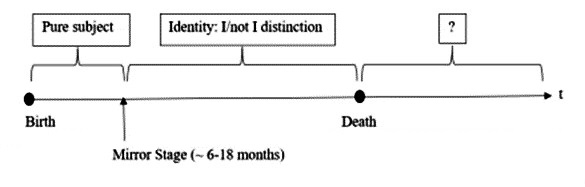
\includegraphics[scale = 0.45]{nathdiagram}
\end{center}
Here,
during the lifetime of the body, the period until the Mirror Stage is
characterized by a lack of identity with the body. Despite the body, the child is pure subject.
This is the period of the Lacanian register of the Real. The Mirror
Stage onwards, there is a misrecognition of the `I' as the ego and the
body, and the I/not-I distinction is created. However, this scenario
assumes the origin of the body (at birth) to be the origin of the
subject, which would imply that the subject is somehow still causally
contingent upon the body. This again raises the question of the
subject's existence independent of the body, i.e. after death. Let us
consider another scenario where the subject, entirely independent of the
body, can precede, and therefore succeed, the body, thereby creating a
timeline such as this:
\begin{center}
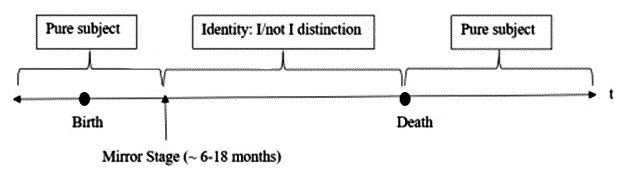
\includegraphics[scale = 0.45]{nathdiagram2}
\end{center}
In this case, the subject exists in time before and after the lifespan
of the body. If the subject and the body are indeed of a substance
dualism, then it can be said that the physical substance of the body
exists for a temporary period in the span of existence of the
non-physical subject. In both the aforementioned scenarios, time has been taken as an external
constant within which the physical body and non-physical subject exist.

In the second scenario, the subject exists indefinitely in both
directions of the timeline. This brings us to the question: What is it
to exist? Is it an experience of time? Does existence necessitate time?
Is `I exist' an experience of a progressing present moment wherein there
is a present in which I am, a past in which I just had been, and a
future in which I will just be? Clearly, this contingence of the
experience of existence upon time is predicated on the fact that there
is a concept of an `I' and that there is a faculty that enables
experience. What happens to existence when there is no concept of an
`I', and no faculty that enables the experience of existence? How can we
say that the `subject exists in time before and after the lifespan of
the body' if it has no concept of an `I' and no body that enables
experience?

On a tangent whose relevance will soon become clear, there arises
another question: if existence is dependent on time, what does it mean,
then, to say that time exists? Does time require an experience of time
in order to exist? Classical physics would consider it unlikely that the
existence of time is dependent on an experience of time (although
according to the theory of special relativity, time is not an absolute---it is something that
exists, the experience of which is relative and flexible). Irrespective
of how it is experienced, both physics and common sense will say: time
\emph{is}. Therefore, if time is an independent entity whose existence
does not depend on any experience of existence, and if the subject can
exist without facilities that enable an experience of existence, then
the subject, like time, is an independent entity whose existence does
not depend on any experience of existence. With this in mind, one can
propose a rather audacious third scenario:
\begin{center}
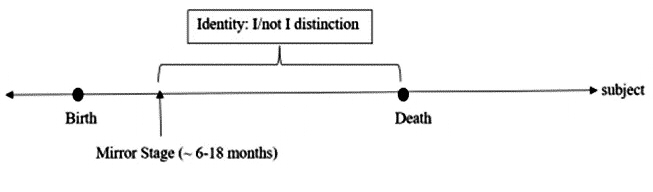
\includegraphics[scale = 0.45]{nathdiagram3}
\end{center}
Here,
the only absolute existence is of the subject. The subject does not
exist \emph{in} time. The subject does not \emph{experience} time. The
subject \emph{is}. The existence of the subject is not dependent on
anything; the subject does not derive its existence from any source.
Entirely self-sufficient, it exists as an absolute, independent
substance. What Lacan calls the Real is the neonatal experience as pure
subject which precedes the Mirror Stage. From the aforementioned
argument about the consequences of death for the subject, the identity,
and the body, we have shown that upon holding Lacan's identity
philosophy true, the existence of the subject can be concluded as
absolute. The Lacanian Real is, in fact, the absolute subject.

A substance duality had been assumed previously which was based on time
as an `external constant within which the physical body and non-physical
subject exist'. Now, since the subject has been shown to be the only
absolute, time is no longer an external constant. The absoluteness of
the subject, therefore, negates substance dualism. There can only be
one, non-dual substance---that of the subject.

It is this non-duality that is the central philosophy of Advaita
Vedanta. The pure subject, the absolute non-dual substance, is termed
`Brahman' in the Upanishads. Adi \'Sa\.nkar\=ac\=arya, the ancient Indian
scholar, summarized the entire philosophy of Advaita in a sentence:
`Brahman is real, the world is an illusion, the self is Brahman itself
and not different' (\'Sa\.nkar\=ac\=arya). The following is the line from his
work \emph{Brahma Jnanavali Mala}:
\begin{center}

\includegraphics[scale = 0.525]{nathBrahma}

\emph{Brahma satyam jaganmithya jivo brahmaiva naparah}
\end{center}
Brahman, the non-dual reality, the `Ultimate Truth', is defined as
\emph{Satyam Jnanam Anantam,} or infinite existence and consciousness.\footnote{\'Sa\.nkar\=ac\=arya 1995.} It is indescribable and ineffable; `one without a
second', it is beyond language, speech, and mind: `The Absolute
Substance or Brahman is beyond space and time, consequently it is
formless and unchangeable\ldots\ it is our true Self'\footnote{Abhed\=ananda
1992.} The Katha Upanishad mentions: `The all-knowing Self was never
born, nor will it die. Beyond cause and effect, this Self is eternal and
immutable. When the body dies, the Self does not die'.\footnote{\'Sa\.nkar\=ac\=arya
1987.} According to Advaita Vedanta, Brahman is the Self (\emph{Aham
Brahmasmi})---the subject---and the sole absolute substance of the
universe: one cannot say it `exists', for it is existence itself. It is
pure existence and pure consciousness: `Consciousness can never be the
object of knowledge. It is always the subject'.\footnote{Abhed\=ananda 1992.}
Therefore, it can be said that Brahman is the same as the absolute
subject previously described.

What both Brahman and the Real seem to signify is a pure,
undifferentiated subject which is `without fissure' and which `resists
symbolization absolutely'.\footnote{Fink 1997, 24; Lacan 1988, 66.} It is an
absolute wholeness or oneness that precedes the Lacanian Mirror Stage
when the subject misidentifies itself as an object: `I', and
consequently divides the plenum into the `I' and the `not-I'. The true
subject is neither `I' nor `not-I'. Vedanta conveys this through the
concept of \emph{neti-neti} (`not this, not this'). It mentions that the
subject is not the `I' and not the `not-I'; however, the subject is that
within which the `I' and the `not-I' arise. Similarly, one can say that
as the Real underlies the realm of reality as constituted by the
Imaginary and the Symbolic Orders---the `I' and the `not-I' of the
Imaginary and Symbolic Orders arise within the Real, i.e. the absolute
subject.

What happens to the pure subject---the Real or Brahman---once identity
is established in the Mirror Stage? Lacan and Advaita Vedanta provide
slightly different answers. According to Lacan, the Real is
irretrievably lost upon entrance into language. The Real is entirely
beyond language: the very signification of it as `Real'---a word in
language---marks our irrevocable separation from it. Lacan would hold
that its signification---as the `Real' or as `Brahman'---makes it
eternally elusive. However, Lacan mentions that the Real, underlying the
realm of the Symbolic and Imaginary, can appear to erupt in guises of
```limit experiences'', namely, encounters with that which is
annihilating, inassimilable, overwhelming, traumatic, or unbearable'.\footnote{Johnston 2018, 13.}

The eruption of the Real is fleeting and incomplete, either pleasurable
(for example, at the moment of orgasm) or traumatic in case of events
that cause the experience of the world to become gravely shaken. In
Seminar XI, he mentions: `Is it not remarkable that, at the origin of
the analytic experience, the real should have presented itself in the
form of that which is \emph{unassimilable} in it-in the form of the
trauma, determining all that follows, and imposing on it an apparently
accidental origin?'\footnote{Lacan 2005, 55.} When the fabric of the Symbolic is
ruptured, the Real seemingly erupts, and it is perceived as traumatic
because it threatens the known and consolidated reality of the `I' and
the `not-I'. Despite that annihilation of the fictive `I' being the very
object of desire, the threatening nature of that destruction and the
fear that it evokes in the individual is the same as the fear of death
and the unknown that lies beyond. Therefore, the individual remains in a
lifelong struggle between desiring and fearing that where the `I' and
the `not-I' are no longer separate, where language and signification no
longer exist; that which is unknown and unknowable; that which is beyond
death.

Advaita Vedanta, however, states that Brahman is never lost---it is
ever present---but we do not realize it due to ignorance\emph{:
`}Though the Self is Brahman, there is not the knowledge of the Self
(being Brahman). That which obstructs the knowledge of the Self is
Ignorance.'\footnote{Harihar\=ananda 2002.} According to the scriptures, Brahman
can be realized primarily through the practice of focused and meditative
\emph{vic\=ara} (discrimination) which allows one to discriminate between
what is truly the Self and what is not.\footnote{Dhire\'s\=ananda 2014.}
Brahman is beyond language, but it can be realized despite language, and
also through language: `\emph{Aum,} the word, is all this\ldots\
\emph{Aum} is the means to the knowledge of Brahman on account of its
having the closest proximity to Brahman'.\footnote{\'Sa\.nkar\=ac\=arya 1995.}

Is it possible to regain the Real or realize Brahman in the lifetime of
the body, once again like the neonatal pure subject? Can the
misidentification of the subject as the object `I', and the subsequent
I/not-I division, be reversed? Can identity ever truly be lost? Is the
ineffable really irretrievably lost when we enter into language, as
Lacan states? Is the only way to enter the state of pure subject once
again (while having the body and sense perceptions, i.e. before death)
to lose language? Let us introduce a thought experiment to consider the
possibilities: Soham is an adult who has lost all their acquired
knowledge of language. Their severe aphasia is a result of acute and
irreversible cerebral damage. Not only are their Broca's and Wernicke's
areas for language production and comprehension in the brain completely
damaged but also their entire store of knowledge and memories of ever
having learnt language has been erased. They are now exactly how they
had been before being introduced into language. However, they still
retain their sense perceptions which allow them to perceive the world
just as before; but the world has no meaning to them since they have no
way of signifying their perceptions such that one perception is
differentiated from another. Now, what should be the impact of this
severe loss on their identity?

Identity, besides being a sense of an `I', is certainly dependent on
memory: the knowledge and events that provide a history to the `I'. The
erasure of all knowledge of language can have a severe impact on Soham's
memories, especially semantic and episodic. It is implausible that
without a process of signification that would allow them to
differentiate perceptions (even memories of past perceptions), Soham
retains the normal memory functions. Therefore, due to Soham's inability
to signify and differentiate objects, their memories can become entirely
redundant. This will have a severe impact on their identity as Soham.
The effect of losing memories on a person's identity is evidenced by
real cases of severe dissociative amnesia; therefore, Soham's
autobiographical identity should, as a result of losing memory function,
also be lost. Having lost a major portion of what defines his identity,
the question now is whether they retain the sense of an `I'.

One possibility is this: since the Mirror Stage appears to precede
entrance into language, it is possible that Soham entirely retains the
sense of identity with the body. The loss of language has no effect on
the consequences of the Mirror Stage they experienced as a child.
Therefore, they are still aware of their bodily integrity. Furthermore,
the loss of language will not hamper their ability to still recognize
their body in a mirror. However, one can be skeptical of this
possibility: how do they identify themselves if they do not have the
faculty of signification? Without any faculty of signification or
learning signification (they do not comprehend when others tell them
that what they see is a mirror, and that the mirror reflects, and that
what they see in the mirror is themselves) seeing themselves in a mirror
would make no sense to them---it would be just another perception that
cannot be signified and differentiated. Still, one can argue that the
effects of the Mirror Stage remain from the memory of the childhood
experience; however, since the loss of language can render episodic
memories redundant, it is unlikely that the memory of the childhood
event will have any consequences on present-day Soham. This scenario,
therefore, is quite unconvincing.

Here, second possibility can be considered. Although Lacan's text of
`The Mirror Stage' seems to suggest that the Imaginary Order precedes
the Symbolic Order, his later emphasis on the role of other human beings
in the process of identification with the \emph{imago-Gestalt} suggests
that the effects of the Imaginary and Symbolic registers occur
simultaneously. The Mirror Stage of the Imaginary Order cannot be
considered to be an event that occurs outside of the influence of
language:
\begin{quote}
if anything, socio-linguistic variables (for instance, the words and
body language of parents) are the causal triggers of the child's
investment in select sensory-perceptual experiences (such as the body
image in the mirror)\ldots{} this means that the imagistic nucleus of
the ego is suffused from the get-go with the destinal ``discourse of the
Other''--- in this case, fateful significations (``unary traits'')
coming from caregivers' narratives articulated simultaneously along with
their encouragements to the child to recognize him/her-self in the
mirror.\footnote{Johnston 2018, 9.}
\end{quote}
It is extremely important to consider that `socio-linguistic
variables\ldots\ are the causal triggers of the child's investment in
select sensory-perceptual experiences (such as the body image in the
mirror)'.\footnote{Johnston 2018, 9.} If language is the very `causal trigger'
for the Mirror Stage, then with their redundant memories and inability
to signify anymore, Soham can be said to have reverted from the
consequences of the Mirror Stage. Not only have they reverted but also
cannot undergo the Mirror Stage event again because the very `causal
trigger' has been taken away. Can it be said, then, that they no longer
have any sense of an `I'? Has the I/not-I divide now been reversed? Is
Soham now purely the absolute subject, despite retaining their body? It
is plausible that through this extreme separation from the Symbolic,
Soham reverts from the effects of the Mirror Stage and Imaginary Order
and resists undergoing the same effects again. With the Symbolic and the
Imaginary removed entirely, only the Real remains. And, Soham has
regained the Real---they are pure subject.

This thought experiment considered the Lacanian view, and it appears
that language is indeed the fundamental factor that determines identity.
The Self as the Real---or Brahman---cannot be regained as long as one
remains in language. The Self shall remain entirely out of reach unless
a person is subject to a loss of language as radical as Soham's. Lacan
points out this elusiveness of the Self due to the established identity
and the faculties of signification in \emph{\'Ecrits:} `I think where I am
not, therefore I am where I do not think. I am not whenever I am the
plaything of my thought; I think of what I am where I do not think to
think'.\footnote{Lacan 2008, 166.} If language binds us in identity, how does one
undo the I/not-I divide and return to the state of pure subject,
according to the Upanishads? Advaita Vedanta advocates for the
realization of the Self as Brahman---pure, non-dual subject---through
the \emph{jnana yoga}, or the way of knowledge. Through knowledge and
rational \emph{vic\=ara}\footnote{Discrimination.}, one can realize the
true nature of the Self. The ancient text of the \emph{Yogav\=asi\d s\d tas\=ara\d h}
mentions:
\begin{quote}
The firm immediate knowledge of the Self arises due to discrimination
by means of \emph{manana}\footnote{Intellectual reflection.} and
\emph{nididhy\=asana}\footnote{Internal contemplation.}\ldots\ By that
discrimination the veil, which causes non perception of Brahman and the
projection, or the reflected consciousness with gross and subtle bodies
and their properties\ldots{} gets obscured and that leads to liberation.
People have their strong ego-identities in their bodies; if such a
strong ego-identity in Brahman comes and obstructs the body-identity, it
is called \emph{immediate} (\emph{aparok\d sa}) and unmoving direct
Knowledge of Brahman.\footnote{Dhire\'s\=ananda 2014.}
\end{quote}
This excerpt suggests that the identity that one feels with one's body
can be replaced by an `ego identity in Brahman'. One can realize this
through wisdom and earnest reflection upon the \emph{vic\=ara} which
allows one to see that the apparent world is not the true Reality.
Focused meditation on the `unreal' nature of the world allows one to
realize that the I/not-I divide is an illusion, and that the Ultimate
Truth is Brahman\footnote{\'Sa\.nkar\=ac\=arya 1995.} The \emph{Yogav\=asi\d s\d tas\=ara\d h}
continues to say that the \emph{jīvanmukta}'s (liberated person) `unreal
worldly behaviors continue, with the help of the false body, senses and
the like' due to his material body.\footnote{Dhire\'s\=ananda 2014.} He continues to
live as he did before his knowledge of the Self as Brahman; however, he
no longer identifies himself as his body---he is aware of the fact that
the `I' and the `not-I' are unreal.

In the \emph{Four Fundamental Concepts of Psychoanalysis}, Lacan
mentions: `it is the subject who introduces division in the individual
{[}habit of saying I{]}, as well as into the collectivity that is his
equivalent {[}others{]}. Psychoanalysis is properly that which reveals
both the one and the other to be no more than mirages'.\footnote{Lacan 2005, 80.}
Vedanta calls `illusion' precisely what Lacan calls `mirages'. What
Lacan says psychoanalysis reveals is precisely what Vedanta says is
revealed through the \emph{jnana yoga}. However, does the knowledge of
Brahman equate to the true experience of Brahman? Is knowledge of the
Real equal to true experience of the Real? Is knowing of the falsity of
the I/not-I divide equivalent to undoing the division?

It appears that realization through knowledge and realization through
experience (like Soham's) are quite different. In the former mode of
realization, one recognizes the I/not-I divide to be unreal but
continues to remain and function in the world without the actual
experience of pure subject. The latter realization is difficult to be
termed as a realization since that would require the ability to compare,
which further requires the faculty of signification. The pure subject
experience of Soham comes at the cost of complete impairment of
functioning in the world. The body becomes irrelevant to Soham;
therefore, the presence or absence of the body should not affect Soham's
state as pure subject. Soham's state before body-death is exactly the
same as their state post body-death. One can say that what they have
achieved in life is precisely what they would have achieved in death.
The knowledge of Brahman---or the Real---entails that one identifies
oneself as Brahman: this can be quite superficial in comparison to the
actual experience as pure subject (like Soham's). To say that one
identifies oneself \emph{as} something, is to employ the faculties of
signification. To say that one identifies as Brahman or the pure subject
is a consolidation of the `I' and the `not-I', not an eradication of the
`I' and the `not-I'---which is what is necessary in order to regain the
Real.

There is much that can be said about the philosophies which speak of the
ineffable plenum---call it Brahman or the Real---which is the  Ultimate
Truth, and that very endless discourse is what makes it elusive. It
escapes us for as long as we can think of it, and it embraces us the
very moment we escape thought. Perhaps, as Lacan and the Vedanta have
said, as long as we have the faculties of signification and the body, we
can only reach as far as knowing that there is something beyond the
illusion of the `I' and the `not-I', and that the Self is greater than
what the ego and the body suggest it to be. Perhaps, it is with
knowledge, that is the consolidation of the `I' and the `not-I', that
one should live numerous peaceful years, and it is in anticipation of
the complete dissolution of the `I' and the `not-I', that one should
welcome death.

\clearpage
\section*{References}
{
\small
\begin{itemize}[label={},itemindent=-2em,leftmargin=2em]	
	\item Abhed\=ananda. \emph{Self-Knowledge}. Ramakrishna Vedanta Math, 1992.


	\item Dhire\'s\=ananda and Sarvadev\=ananda. \emph{Yogav\=asi\d s\d tas\=ara\d h}. Sri
Ramakrishna Math, 2014.


	\item Evans, Dylan. \emph{An Introductory Dictionary of Lacanian
Psychoanalysis}. {Hove: Brunner-Routledge}, 2003.


	\item Felluga, Dino F\emph{.} ``Modules on Lacan: On the Structure of the
Psyche.'' \emph{Introductory Guide to Critical Theory.} Purdue University, January 31, 2011.

	\item Fink, Bruce. \emph{The Lacanian Subject: between Language and
Jouissance}. Princeton University Press, 1997.

	\item Harihar\=ananda, Sarasvat\=i. \emph{Advaita Bodha Deepika, the Lamp of
Non-Dual Knowledge}. Sri Ramanasramam, 2002.

	\item Johnston, Adrian. ``Jacques Lacan.'' Stanford Encyclopedia of
Philosophy. Stanford University, July 10, 2018.

	\item Lacan, Jacques, and Jacques-Alain Miller. \emph{The Seminar of Jacques
Lacan}. Norton, 1988.

	\item Lacan, Jacques, et al. \emph{The Four Fundamental Concepts of
Psychoanalysis}. W. W. Norton \& Company, 2005.

	\item Lacan, Jacques, et al. \emph{\'Ecrits: a Selection}. Routledge, 2008.

	\item \'Sa\.nkar\=ac\=arya, Acarya, Gaudapada,. \emph{The Mandukya Upanishad: with the
Karika of Gaudapada, and the Commentary of Sankaracarya}. Advaita Ashrama,
1995.

	\item \'Sa\.nkar\=ac\=arya. \emph{Katha Upanishad}. Advaita Ashrama, 1987.
	
\end{itemize}
}
\addtocontents{toc}{\setcounter{tocdepth}{1}}

\essayheader{Intentionality's Role in Bringing Art to Life}{Nathan Fish}{University of California, Los Angeles}
\fancyhead[LO]{\scshape Intentionality's Role in Bringing Art to Life}
\fancyhead[RE]{\scshape Nathan Fish}

\addtocontents{toc}{\setcounter{tocdepth}{0}}
\pretolerance = 400
We often say of art, `It seems as though it's coming to \emph{life}
before me!' This is an aesthetic judgment---it requires a sort of
sensitivity and attention to qualities different from a normal or
descriptive attitude toward objects. I will term the aesthetic property
attributed in this judgment \emph{livingness}; to say of an object that
it comes to life before you is to attribute livingness to it. This essay
explores what specifically is happening when we say of art that it
appears living to us, with the explanation proceeding via psychological
and representational capacities of the viewer or reader. My main
argument will be that an experience of the artist's
\emph{intentionality} can play a large role---though certainly not the
only role---in having an aesthetic experience of livingness. My primary
case will be poetry as, in spite of its long and weary history with
intentionality and the use of the term in literary analysis, it is the
art form in which an author's psychology is most exposed---which is
likely why it has caused so much trouble.

To these ends, I will first explicate the terms \emph{livingness} and
\emph{intentionality}. I will address the former in the first section
and clarify precisely how livingness functions as an aesthetic concept
in Frank Sibley's sense.\footnote{Sibley, ``Aesthetic Concepts''.} The
second section will then explain intentionality and how it relates to
livingness. This will be connected to experiments in developmental
psychology which show how attributing life and intentions to objects is
a natural and fundamental psychological capacity. I will further push
this connection as it pertains to art in the contrast between what is
cliché and what is original, as it is in originality that authorial
intention becomes most evident and makes a poem seem most alive.

\section{The Aesthetic Concept of Livingness}


As stated, I use the term \emph{livingness} to mean the quality someone
is attributing when they say, in the aesthetic sense, that something
appears living to them.\footnote{It might seem that inventing the word
  \emph{livingness} just serves to unnecessarily obfuscate the matter.
  This is not the case; there really isn't another word that properly
  captures the judgment ``coming to life'' in the noun form. Words like
  \emph{lively} are too linked to ideas of joyousness or spring-like
  themes, which are not necessarily related to livingness. Indeed I
  think poetry, and art as a whole, can come to life to a subject when
  it is deeply still, eerie, morose, and so on.} It's an odd term --
rarely ever do people say `this painting has livingness'; they'll rather
say `this painting is living' or `this painting appears to be living'.
But for reasons soon to be discussed, it is important to distinguish
livingness from common conceptions of what is merely \emph{living,} as
this word can be construed in a non-aesthetic sense (namely, a
biological one)\emph{.} As such, I will use livingness when speaking of
the \emph{aesthetic} attribution of living.

Since livingness is a term used to convey an aesthetic judgment,
livingness is an \emph{aesthetic concept}. In his essay ``Aesthetic
Concepts'', Frank Sibley formulates a schematic definition of the term.
He writes an aesthetic concept is ``a word or expression such that taste
or perceptiveness is required in order to apply it\ldots''\footnote{Sibley,
  1.} I will explain more of Sibley's view below, as I think he is spot
on in his understanding. Presently however, I hope to expand this rough
outline in ways he does not, as it will help flesh out our understanding
of how aesthetic experiences and concepts function.

I take ``taste or perceptiveness'' to specify the certain way in which
we represent objects aesthetically. It is a different attitude than that
of a descriptive, or ``existential'' attitude, in the words of
Husserl.\footnote{Husserl, ``Letter to Hofmannsthal''. In one of his few
  mentions of aesthetics, Husserl compares the aesthetic attitude with
  the phenomenological attitude, in that both are concerned with how
  objects appear. This is contrasted with the ``existential'' attitude,
  which I will usually term ``descriptive'' or ``normal'' to avoid
  unnecessary confusion.} Descriptive attitudes are concerned with
\emph{what} an object is, and lead a subject to connect their
representations to some degree of actuality and objectivity in the
world. When concerned with aesthetics, however, we can roughly say the
attitude is an imaginative, interested, and perhaps pleasant or
otherwise emotionally significant approach to experiencing an object.
This attitude is less concerned with what an object is but more so how
it strikes us. Thus, I'll say the experience of livingness, i.e., `this
is coming to life!', is an experience of this aesthetic nature. For
example, you might say it of a mountain because it is poised stalwartly
on the horizon, ``greeting'' the sunrise.\footnote{Citing only pleasant
  and appreciative experiences such as these would mischaracterize the
  complexity of aesthetic experiences. For example, when things come to
  life in, say, genres of horror, such as a haunted forest or an
  uncannily life-like doll, it can be quite disturbing, but nonetheless
  striking and capture our interest. This further specifies that
  aesthetic experiences are not merely what are \emph{pleasing} to us or
  to our taste, but something that pierces us and demands attention in a
  way different than a descriptive attitude toward the world.} In this
way we personify the mountain, attributing intentions (of course, we are
not speaking of any artist's intentions in this case yet) based on how
it appears to us, making it seem as though it possesses livingness.

It is illustrative to provide an example of \emph{living} in the
non-aesthetic sense; this contrast will bring to light a number of
points that differ between the aesthetic and descriptive attitudes. The
non-aesthetic representation of living is a descriptive fact,
attributing the basic feature of living to an object due to the way it
behaves in the world.\footnote{This alludes to the experiments in
  developmental psychology that will be covered later (Simion et. al.,
  ``A predisposition for biological motion'') demonstrating the
  fundamental capacity we have in identifying objects that show
  life-like qualities, or ``biological motion'' in their words.}
Attribution of just ``living'' can be uninterested and unsurprising, or
quite surprising indeed, yet in a different sense than an aesthetic one.
For example, you might think it of a lizard because of its endogenous
motion and responsiveness to the environment---no one would find this a
surprising attribution, except for perhaps a young toddler who had never
seen a lizard. However, attributing ``living'' to something (in the
non-aesthetic sense) that is \emph{not} living can be surprising or
interesting, such as a hat that seemingly floats of its own accord. In
this case it would be incorrect to believe and say `this is living';
rather, we would say `this \emph{appears} to be living'. Yet this is
\emph{still} different from saying `this has livingness' or,
equivalently, `this appears living \emph{in the aesthetic sense}.'

An example that teases this apart fully is as follows. Imagine that two
viewers behold a painting in a museum. One comments, `Isn't it amazing
how it just comes to life before you?' This is clearly an aesthetic
judgment attributing the term livingness, which could be explained in
reference to some characteristics in the painting. Before the other can
reply however, at just that moment the painting actually begins to slide
along the wall in a zig-zagging motion seemingly by its own volition --
let's say because of some contraption an impish museum curator
installed. At this moment the viewers might judge that the painting
certainly \emph{appears} as though it is coming to life (at least for a
few fractions of a second), but they do this in the non-aesthetic,
literal sense. This may be surprising to the viewers, yet it is still
unlikely they would believe the painting really is alive. They would
search for a cause, such as the contraption moving it.

The two judgments differ in ways that are illustrative of the difference
between the aesthetic and non-aesthetic. The first way they differ is
that they point to different facts about the object. One picks out
certain characteristics in the work that are of aesthetic interest to
the viewer; the other picks out the spontaneous motion of the painting.
Second, the aesthetic attribution of livingness does not require any
sort of belief in how the thing actually is---indeed you suspend
disbelief to talk about such judgments. Yet the case of the painting
literally moving requires the viewers to search for an explanation as to
why the painting is not \emph{actually} living. Further, while the
aesthetic case is appreciative and delightful because it contradicts
expectations, the non-aesthetic case would be upsetting and disturbing
for the same reason! Thus, there are meaningful and distinct ways in
which the attribution of living might be used in the aesthetic or
non-aesthetic sense.

You'll note that this exposition has often pointed to the fact that we
attribute livingness \emph{because} \emph{of} some perceived or
represented characteristics. Indeed, when Sibley speaks of aesthetic
concepts requiring ``taste and perceptiveness'' it is necessary that
there are some characteristics of the object that provide the basis of
this exercised taste or perception. This prompts the question: on what
basis or in reference to what characteristics do we employ the concept
of livingness\emph{,} or all aesthetic concepts for that matter? What
qualities contribute to or cause such experiences? It seems fairly
obvious how we attribute living---we judge based on its capacity for
internal motion, whether it grows, if it reacts to its environment, etc.
It's clear given any object (with the exception of the odd case here and
there, like a virus) that we could determine it living or non-living.
This is not so when determining livingness.

To return to the works of Sibley, this is not an easy issue to resolve.
Sibley argues that aesthetic concepts are hardly ``condition governed'',
that is, they are not the sort of concepts that are decided by necessary
or sufficient conditions.\footnote{Sibley, 4.} There is no formulation
in which one can say `If $X$ possesses the aesthetic concept $Y$, it will
necessarily follow that it has characteristics $A, B, C$, and so on' nor
is there a formulation `If $A, B, C$, etc., are present, then $X$ possesses
the aesthetic concept $Y$'. Therefore, we do not have a complete catalog
of characteristics that we can readily point to such that we decide the
case that something has livingness (or is joyous, or tortured, or warm,
and so on). Indeed, characteristics that might be said to commonly lead
one to judge an object to have some aesthetic quality can deny that
judgment in another object. A pertinent example Sibley provides is when
he writes, ``One poem has strength and power because of the regularity
of its metre and rhyme; another is monotonous and lacks drive and
strength because of its regular metre and rhyme.''\footnote{Sibley, 7.}

Nonetheless, we can say that there are some characteristics that can
\emph{likely} connect to an aesthetic concept. For example, orange and
red shades found in sunsets are likely to characterize a painting as
warm. To return to livingness and poetry, I argue that an
author's intentionality, especially when exercised in an original and
novel way, often counts for and not against livingness in the Sibleyan
sense. You should always keep in mind, when it is not explicit, that
this is no guarantee. Indeed, if an author intends to write a poem that
is entirely formulaic or unvarying from the cliché, or a poem that has
no adherence to structure and poetic conventions, it is very likely the
poem will seem \emph{lifeless} or too disorganized to be a coherent,
living thing. Intentionality is no decisive factor that a poem possesses
livingness. Before I draw these connections, however, it is time to
clarify precisely what I mean by intentionality in this context.

\section{Representations of Intentionality}

When speaking of a reader's representations of an author's
intentionality, I will have four distinct notions in mind. I believe a
reader can represent all four notions of intentionality when reading a
work (or viewing other forms of art), sometimes stratified, sometimes
blended together. When reading, we can certainly form ideas about 
	\begin{enumerate}
		\item the
general mental contents of the author, either presented in the work or
underlying it; 
		\item what the author \emph{meant} while writing; 
		\item their goals to communicate their meaning; and 
		\item what moods and
phenomenological states they underwent while writing, what writing it
was \emph{like}.\footnote{This use of phenomenology is in a fairly
  standard sense: ``Phenomenology is the study of structures of
  consciousness as experienced from the first-person point of view''
  (Smith, ``Phenomenology'').}
  \end{enumerate}
We can state these representations as
unspecified descriptive facts about the work. For example, we might say
or think `the author had some mental contents while writing this' (this
is in the first sense) or `the author had some conscious experience of
these mental contents in a certain way while writing this' (in the
fourth, phenomenological sense). When we do this, we are certainly
pointing out objective facts relating to the work.\footnote{There are of
  course fringe cases in which we would be \emph{mistaken} to do so,
  such as if a robot randomly generated a poem, or some ant accidentally
  tracing a haiku in the sand. I am not so interested in these
  complications; I am dealing with typical poetry and artwork in which
  intentionality is some constitutive feature of the work, i.e., it was
  made by someone.} However, when we interpret the intentionality or
regard it in an aesthetic attitude---that is, approach it in an
imaginative and curious manner, interested in how it \emph{seems} to us
-- this is when we represent intentionality as an aesthetic
characteristic. For example, if we were to say, `the author must have
been reminiscing of his mother' or `it is clear through his tone that he
voiced this with deep passion and pain', we place our own interpretation
on the latent intentionality in the work and form aesthetic judgments on
these grounds.

I believe it is these interpretive representations of intentionality
that contribute, in some cases, to an aesthetic experience of
livingness\emph{.} When a reader represents intentionality, especially
in the phenomenological sense, they may feel as though the author is
coming to life through their work. This can come about in many different
ways, of which I will only discuss a few to provide sufficient examples.

The first is when one connects with the emotions they believe are
portrayed in the poem (through the speaker, the tone, the diction, etc.)
and attributes them to the author's intentionality. In such a way they
might be attributing all four uses of intentionality above. The reader
can imagine the following beliefs distinctly or in conjunction: 
	\begin{enumerate}
		\item the
author was feeling \emph{x} or thinking of \emph{x} while writing;
		\item the author meant to communicate they were feeling \emph{x} or thinking
of \emph{x};
		\item the author conveyed \emph{x} to make us feel \emph{y} or
to make the poem seem \emph{z};
		\item writing of \emph{x} must have been
like or felt like experience \emph{y}.\footnote{It is worth specifying
  here and later that the reader doesn't need to be correct about their
  representations of the author's intentionality to have an aesthetic
  experience. Indeed the author could have been feeling joy or relief
  when voicing something tragic---or they could have felt indifferent
  and smug, just hoping to bag some money through their flowery words.
  Whether or not a reader ``gets it right'' in their interpretation has
  no bearing on their appreciation of a work. To further complicate the
  matter, the reader could even imagine the author meant to have such
  insincerity, that the author is cleverly disguising their emotions or
  speaking through some character's voice for dramatic effect. These
  representations can also enhance or detract from the aesthetic
  experience of livingness in a poem.}
	\end{enumerate}
These beliefs might lead the
reader to regard the author as a friend, a confidant, a suffering
companion, and so on. They are moved to empathize or sympathize with
these emotions or thoughts they believe the author had. As a result, the
attributed livingness in the poem is due to the reader having a genuine
and organic experience with a seemingly living entity, communicating
with them as they would with the people around them.

In a second case, a reader can be impressed by the brilliance or
expertise of the poet, making judgments such as `the way in which they
describe the scene makes it come to life before me' or `their cutting
language pierces through me'. In these ways, we might say they are
representing the author's intentions to \emph{be} understood and to be
seen as an artist. By fulfilling this imagined desire of the author, the
reader has a pleasant or emotional experience in this mutual
communication and understanding. In these two cases, the intentionality
is explicitly and immediately represented, becoming a primary
contributing factor to the experience of livingness. It is an experience
more common in confessional and Romantic poetry, in which the author has
full expressive power and is received as such by their audience.

\pretolerance = 100
But what of poems that don't put the spotlight on the poet? This more
complex example is when we experience livingness and it is not
\emph{immediately} in virtue of the author's intentionality. In this
case there are other elements in the poem that appear living; it seems
most common when the poem surprises us and deviates from a cliché that
it springs to life. I argue this surprise can lead us to \emph{search}
for what caused the poem to jolt us so, which leads us to the author's
intentionality as the ``animating force'', so to speak. It leads us to
puzzle over what they meant, what they were thinking as they wrote, and
whether they meant to surprise and delight us. This phenomenon will
require more explanation, and I think it will be best to draw a
comparison once again between attributing living in the non-aesthetic
sense and livingness. This comparison will be centered on studies in
developmental psychology, particularly the work of Simion et.
al.\footnote{Simion et al., ``A predisposition for biological motion''.}
and Luo \& Baillargeon.\footnote{Luo and Baillargeon ``Can a
  self-propelled box''.}

Simion et. al. have determined that infants attribute what they call
\emph{biological motion} as early as two days old (likely to be innate)
with very minimal conditions.\footnote{See note 11.} When shown animated
dots on a screen in the shape of moving animals (in this case, a dotted
outline of a walking chicken), the infants show a preference and
interest in what appears to have biological motion over displays that
show random motion not organized in animal shapes.\footnote{This is of
  course to say they show preference and interest in the
  \emph{descriptive,} not \emph{aesthetic} sense. While we usually talk
  of preference and interest in an aesthetic sense, it's understandable
  that an infant would have interest in a descriptive attitude because
  everything is novel and surprising to them.} It of course would be too
far to say the infants ``represent'' something as complex a concept as
``living'' at this stage. Nonetheless, this example demonstrates just
how fundamental and natural it is for us to see something as living and
take interest in it.

Now we can take this further and see how biological motion figures into
\emph{goal attribution}. In Luo and Baillargeon's study, they found that
infants as young as 5 months old expected a self-propelled box to have
``preference'' for the object it was shown to move toward and touch
versus an object that the box had not moved toward.\footnote{See note
  12.} They would be surprised if, when the objects' positions were
switched, the box moved toward and touched the object it hadn't been
previously seeking. Again, it is too far to say the infants develop
representations of intentionality from this. Nonetheless, we can reason
that the infants attribute some sort of rough goal to the
self-propelling box, that the box ``prefers'' or seeks out an object. We
can use this to explain how we detect intentions and goal-setting in the
non-aesthetic sense. It is very natural as adults, even when we know
better, to imagine an object to have life and intentions when it
exhibits some sort of endogenous motion and consistent action.

Here's how we can connect this to aesthetic experiences in poetry. As
explained above, one of the simplest criteria for representing something
as living (and further, attributing intention) is that it can exhibit
biological motion, i.e., self-propel, move without outside forces or
even act against outside forces. Let us then equate common poetic
structure, such as a sonnet, with regular, non-organic motion, like a
ball rolling down a ramp. Imagine an author who takes the structure of
the sonnet and then, with an utter lack of inspiration, formulaically
plugs in words to compose the sonnet. They make trite rhymes such as
`fly' and `high', `love' and `dove'. They write about an over-worn
theme, such as their beloved. Their volta is awfully bland, predictably
lamenting over how their love was spurned. In no way do they vary from
the sonnet tradition, written and rewritten for hundreds of years. It's
very likely that to one who has read a few sonnets, this poem will seem
to be dull and \emph{lifeless;} it will fail the conditions needed to
have the aesthetic quality of livingness. Rather, it will fall with an
uninteresting thud, like a rock dropped from a balcony. There is no
variation in the law-like motion. Now, if a rock were to turn around and
vengefully return to the one who dropped it, scoring a nice bruise on
their brow, this certainly would be cause for surprise. We might imagine
that the rock was \emph{living,} and had a rather spiteful goal or
intention.

In this sense, a poet who varies from the scheme of a poetic genre does
exactly this. In creative strokes they intervene in the predictable
motion of the poem, interjecting slant or off-rhymes, varying the
syllables or spacing, enjambing lines or breaking them abruptly. These
variations surprise the reader, and stand out as distinct experiences,
notably differing from the ``non-biological'' motion of unoriginal
poetry. The poem seems as though it comes to life in this way. This
surprise prompts the reader to think about what \emph{causes} such
surprise, which can lead them to the author.

An artist's intentionality is most noticeable to the reader when they
break clichés or norms. A reader can choose (or intuitively be led) to
represent these moments of intentionality in the aesthetic and
interpretive sense. They engage with and playfully imagine what the
author's psychological state might have been when introducing these
unique and idiosyncratic moments. The reader may feel \emph{as though}
they're peering into the head of the author. As such, they have an
aesthetic experience of livingness, constituted by two experiences. The
first is the initial surprise when the poem varies from what the reader
expected, making it seem ``alive''. This surprise can lead one to
attribute this to the author, at which point they represent and engage
with their intentionality as though they were still living.

With all the pieces set, we are now ready to see this aesthetic
experience in practice. I will examine two analyses of sonnets, both of
which are centered on the author's use of enjambment to break cliché
sonnet structure. Enjambment is when, in a poem, two separate lines run
together without pause, such as if it lacks a comma or the clause is
only completed by reading on to the following line. My goal in citing
these analyses will show how a reader can notice the specific techniques
an author uses to break clichés and surprise them, prompting the reader
to reflect on the author's intentionality. I will further argue that the
reader's capacity to do so enables them to judge the poem on the grounds
of the aesthetic concept of livingness, and that this phenomenon
contributes to their aesthetic experience of the poem as a whole.

\section{Two Cases of Intentionality Experienced Through Enjambment}

In Hobbs' book \emph{Literature and Cognition,} he applies coherence
theory and discourse analysis used in cognitive science and AI research
to the understanding of literature. He analyzes ``Sonnet 20'' by John
Milton, often referred to as ``Lawrence of virtuous father virtuous
son''. His review is quite thorough and splits each line into two or
three segments; as such, I will only deal with his analysis of two
lines, 5 and 6, that will suffice to illustrate that paying attention to
the intention of the author does yield fruitful discussion and aesthetic
representation. His focus is to use these lines to argue for an
interpretation of the meaning of the poem. My goal is to use his
insights to demonstrate that such sensitivity to the intention of the
author contributes to an \emph{aesthetic} experience. The two lines in
question are 5 and 6, and I've included the first four to give context.
I also recommend settling in to a space of receptivity and thoughtfully
engaging with the poem---the attitude of reading philosophy can often
detract from an aesthetic one:

\begin{quote}
{\parskip = 0em
Lawrence of virtuous father virtuous son,

\hspace{1em} Now that the fields are dank, and the ways are mire,

\hspace{1em} Where shall we sometimes meet, and by the fire

\hspace{1em} Help waste a sullen day, what may be won

From the hard season gaining; time will run

\hspace{1em} On smoother, till Favonius re-inspire
}
\end{quote}

The first four lines of the poem provide the setting and characters: the
speaker and the one he addresses are facing a harsh winter (the ``hard
season gaining'') and sometimes meet by a fire to spend leisurely time
together. It seems that the semicolon in line 5 above concludes the
discussion and establishment of time, place, and the meeting of the
characters. In this context, the statement ``time will run'' is a stoic
and bleak statement about the season; Hobbs writes, ``The reader's first
impression is that the same idea is being repeated and
emphasized.''\footnote{Hobbs, 121.} However, once they proceed to line
six the reader realizes that line five and six are enjambed, and
withholding a comma until ``smoother'' suggests the complete clause is
``time will run on smoother''. This changes the interpretation to the
exact opposite of what one first expects. The statement ``time will run
on smoother'' is a wishful and expectant statement rather than a bitter
one. The characters hopefully await until Favonius (a Roman god of
spring) reinspires the earth.\footnote{Hobbs, 120-121.}

This change in the interpretation surprises a reader. By varying from
the traditional sonnet structure in which each line pauses at the end
and contains a complete clause (see lines 1 and 2 as an example), Milton
lulls us into believing that this poem will follow standard, law-like
sonnet structure. However, he anticipates this and plays off of our
expectations. He varies the lines and makes the poem seemingly ``jump''
out of this uninteresting progression, analogous to something with
endogenous, biological motion. This captures our interest, as we are
naturally predisposed to take interest in things that appear living.

It is clear that what underlies the reader's shift in interpretation is
their grappling with what the \emph{author} meant. One thinks Milton's
meaning is to reinforce the theme of the poem, but he really intends to
introduce the turning point with the enjambment from lines 5 to 6. We
might ponder over what he was thinking and feeling when writing this, if
he hoped a clever reader would notice and delight in this move, if he
anticipated our surprise at this moment. This is where the aesthetic
experience of livingness is reinforced in the context of intentionality
and we pleasurably connect with the poem in a distinct way. By
representing this intentionality, we might feel as though we share in
communication with Milton, like we understand some private, clever
utterance he shared with us. Hobbs sums up this sentiment in one of the
very last statements in his book: ``Then what distinguishes poetic
discourse is not so much the shape of the work that the writer executes.
Rather, it is the special relationship he establishes with his reader,
demanding the best of both writer and reader, communicating important
insights, and demonstrating the depth to which we are
understood.''\footnote{Hobbs, 171.}

Let us examine another case then, this one presented in Timothy Steele's
\emph{All the Fun's In How You Say a Thing.} This will focus less on the
surprising aspects of a poem, but on a poet's use of enjambment to match
up with the sensory qualities of the poem. This reinforces the analogy
between the perceptual and physical attribution of \emph{living} and the
metaphorical representation of livingness\emph{.} The poem in question
is Browning's ``My Last Duchess''. Steele writes, ``In most instances,
he {[}Browning{]} uses the run-ons {[}enjambment{]} to suggest
rhythmically the thing he is describing. For example, when he writes

\begin{quote}
The bough of cherries some officious fool\\
Broke in the orchard for her\ldots{}
\end{quote}
the enjambment---the breaking of the pentameter over into the next
verse---serves as a rhythmical analogue to the activity of the
branch-snapper.''\footnote{Steele, 99.} When we read such descriptions
in a poem, indeed we imagine the scene before us and engage in sensory
representation. This may be enough to constitute some experience of a
scene playing in a life-like manner before us. However, such
representations are enhanced and focused by literary techniques such as
the one described. Poems do not just convey scenes through words; poets
control the spacing, meter, and punctuation in ways unique to the art
medium such that they parallel what is being said. When a reader
represents the poet's intentionality such that the poet purposefully
employs these techniques, there's an additional layer of livingness
appreciated. The reader might feel as though they're in private and
subtle communication with another's brilliant mind, working with the
author to construct meaning.

Steele presses on and cites a few more lines in which Browning employs
this technique. This analysis centers on the phenomenological
representation of intentionality. He quotes the lines:
\begin{quote}
\ldots all and each\\
Would draw from her alike\ldots{}\\
and when he refers to the calling of\\
\ldots that spot\\
Of joy into the Duchess' cheek\ldots
\end{quote}
and follows it with commentary: ``the enjambments convey the Duchess's
warm responsiveness to---and her spontaneous and candid delight in --
the world around her. Reading these lines and reading through their
turns, we may remember getting off a plane or a bus and catching sight
of someone we loved whose eyes lit up and whose face blushed happily to
see us.''\footnote{Steele, 100.} We have representations of
intentionality in many layers in this analysis. First, the most
immediate representation, and the one provided by Steele is of the
\emph{character's} phenomenal states---the Duchess. Her mental states
are being directed in such a way as being joyous, ``warm'', delightfully
regarding her environment. We enter into an empathetic state and share
in the Duchess's way of seeing the world, leading to an aesthetic
experience of not only, say, joyousness\emph{,} but of livingness
\emph{as well,} in that we feel we are relating to a character coming to
life before us.

However, this intentionality is not of the author's; it is of the
fictional character or the poem's contents. We connect with Browning's
phenomenal states when we represent him thinking of such a beautiful
sight---perhaps he thinks of his wife, or a love from his youth. We
feel his excitement and heart ache, sharing again in an empathetic state
in which we feel as though we connect with the author in mutual
understanding. Finally, we have a representation of intentionality in
the second and third sense (as described in Section II), as in Hobbs'
example above. We take notice of Browning's enjambment and see how he
ran these lines together to convey this passionate regard for the world
expressed by both the Duchess and the speaker. We can delight in this
manipulation and appreciate it, producing yet another representation of
livingness derived from the author's intentionality.

\section{Some Counterarguments and Their Responses}

In what has been said above, I have shown that livingness is a specific
aesthetic quality that captures the sentiment of when something comes to
life (in a non-literal, aesthetic sense) to someone. I have further
argued how intentionality ties into livingness, particularly using
examples in which the author's intentionality serves as an ``animating
force'' so to speak; their manipulation of a reader's expectations
surprise us and impress us, making the poem seem as though it is a
living, acting entity. I illustrated this with analogies to biological
motion and attributing intentionality to non-living, moving objects,
which seems parallel to attributing intentions to art that surprises us
and varies from law-like, inorganic, cliché motion.

In the examples I have given, one could certainly point out that the
author's intentionality does not \emph{need} to be represented at all to
have these experiences of livingness\emph{.} A few scenarios could show
situations in which this is the case. A reader may skim through the poem
and not take notice of any of these technical literary elements. They
could be, at worst, disinterested in the poem and have no aesthetic
experience. In a slightly better situation, the reader takes note that
the poem indeed felt a little ``alive'' to them, but can't put their
finger on exactly why. With a yet more sophisticated experience, the
reader might have a reaction to the livingness and cite qualities that
are \emph{not} attributed to the author's intentionality, such as the
life-like and realistic descriptions, or strictly the intentionality of
the characters in the poem. It is true that aesthetic experiences are
often immediate and emotional, and to accurately describe what is
happening when we have such experiences, it may be unnecessary to
reference these sorts of intellectual and interpretive filters.

I do not need to refute the possibility of these counterexamples to
still conclude what I have thus far. The instances of other aesthetic
experiences do not deny our capacity to render the particular judgment I
have explicated here. Nonetheless, running through each of these other
cases might elucidate some clarifying points. The first case in which
someone is entirely unimpressed does not require much discussion. As
Sibley writes, ``\dots a man need not be stupid or have poor eyesight to
fail to see that something is graceful. Thus taste or sensitivity is
somewhat more rare than certain other human capacities; people who
exhibit a sensitivity both wide-ranging and refined are a
minority.''\footnote{Sibley, 3.} This is not to commit to some elitism---Sibley argues that most people employ aesthetic concepts in day to
day life. However, it does require some experience and knowledge to
point to what makes a poem good or bad, and further I believe it
requires the right disposition. If one thinks poetry is a waste of time
altogether, they will be ruling themselves out of such experiences. If
someone is tired, hungry, stressed, has been reading for too many hours,
etc., then regardless of their aesthetic sensitivity, they may miss a
nuanced judgment they would have otherwise had.

I can treat the second and third counterexamples at the same time. My
first point of defense is that if one does not reference the author's
intentionality but nonetheless has an aesthetic experience, this in no
way denies their capacity (or anyone's capacity) that they \emph{can}
represent authorial intentionality. Someone who does not make this
connection in one poem might see intentionality as a contributing
characteristic in another, or when revisiting the same work come across
this discovery.

My second point is that even if someone does not know why they feel as
though a poem is alive, or if they cite characteristics other than
intentionality, this does not exclude the possibility that authorial
intentionality was an \emph{implicit} factor in their judgment. Indeed,
a critic might explain to this reader why they believe the author's
intentions are what animate the poem, and the reader could say, `Yes!
That's exactly it' or `I hadn't thought about that, but when you put it
that way, I certainly agree.' It would be too strong for me to argue
that therefore authorial intentionality \emph{always} implicitly
underlies these sorts of judgments---this is not the case. We must keep
in mind Sibley's argument that there is little that is logically
guaranteed or necessitated in aesthetics. There is nothing wrong with
having aesthetic experiences of livingness that do not involve
intentionality. Nonetheless I have made a case for why and how we can
have these aesthetic experiences, and I further hold that these
judgments are not uncommon due to our fundamental predispositions to
personify and imagine things to be alive.

Now, if you take little interest in the world of aesthetics or
literature, this may seem like an unimportant or modest claim. So I have
established what it's like to have an experience of livingness,
the way in which we represent such experiences, and how intentionality
can play a major role in contributing to this phenomenon. What of it? I
have three responses to this cynicism. The first is that this is a move
in arguing, in small steps, for a valid place for intentionality in
aesthetic experience. Prejudice against intentionality is still alive,
usually in pop or overzealous interpretations of ``The Intentional
Fallacy'' or other New Criticism era thought.\footnote{Wimsatt and
  Beardsley, ``The Intentional Fallacy''.} However, my argument lives
comfortably within the conceding points of anti-intentionalists, of whom
Lamarque writes, ``Indeed Wimsatt and Beardsley readily admit that an
author's `designing intellect' might be `the \emph{cause} of a poem';
they deny only that it is a \emph{standard} for judging the poem. Also
they are happy to acknowledge intentions \emph{realized} in a
work.''\footnote{Lamarque, \emph{The Philosophy of Literature,} 119.} My
thesis is a specification of \emph{how} intentions are realized in a
work, and the aesthetic impacts they have. As such, I see this as
elaborating on the common ground and showing how intentionality can
function in interpretation and aesthetic experience even in a post New
Criticism era. Further, I do not argue that this use of intentionality
is a ``standard'' for judging a work. I am merely pointing to the fact
that we \emph{do} have such representations, and that these \emph{can}
figure into our appreciation of the work. It may be that one wishes to
exclude these sentiments in formal critique, that citing intentionality
when analyzing a poem will lead one astray due to subjectivity and the
elusiveness of ``really'' knowing an author's intentionality. This is
fine in those contexts, but when our goal is to describe how experiences
of livingness (and other aesthetic qualities) work, it is disingenuous
to count intentionality out.

My second claim is that this is a model exercise in approaching
aesthetics. Despite our strivings, the realm of aesthetics is not yet a
mastered frontier, let alone a coherent and well-explained sphere of
human thought. It is hard to get specific about how we make aesthetic
judgments and what their nature is. We should not appeal to universal
principles as the classical, medieval, and early modern tradition did.
Historically, this gets us more turned around than clear about the
matter. We ought to provide examples that can be understood and are
common to our experiences---building a bottom-up theory of aesthetics.
This essay is the long version of one such example.

Finally, my third response is less philosophically established, but a
belief I hold dear to my heart. Paying attention to how we personify and
have a unique capacity for imagining and sharing meaning with others
promotes an appreciation and recognition of beauty in the world. As
Hobbs writes, ``Much of what is most powerful in literature is a
conjunction of the two categories---the fictional narrative. It is an
author's invitation to the readers to a mutual imagining, to delight and
instruct, by the creation of a possible world and possible characters
striving toward goals, told in a way that directly reflects our own
experience as we plan our way toward our goals in a world that denies us
so much of what we desire.''\footnote{Hobbs, 40.} Explaining how
intentionality functions to deliver livingness can give one a heightened
sensitivity in employing this capacity. So I invite you, mutually
imagine and delight in the intentions of others and the world around
you, fictional or not. It may just serve to increase your appreciation
for what surrounds you.


\clearpage
\section*{References}
{
\small
\begin{itemize}[label={},itemindent=-2em,leftmargin=2em]	
\item Hobbs, Jerry. \emph{Literature and Cognition}. CSLI, 1990.

\item Husserl, Edmund. Letter to Hugo von Hofmannsthal. ``Letter to
Hoffmansthal.'' Göttingen: Göttingen, January 12, 1907.

\item Jacob, Pierre. ``Intentionality.'' Stanford Encyclopedia of Philosophy.
Stanford University, February 8, 2019.

\item Lamarque, Peter. \emph{The Philosophy of Literature}. Blackwell, 2009.

\item Luo, Y., and R. Baillargeon. ``Can a Self-Propelled Box Have a Goal?:
Psychological Reasoning in 5-Month-Old Infants.'' \emph{Psychological
Science} 16, no. 8 (2005): 601--8.

\item Sibley, Frank. ``Aesthetic Concepts.'' Essay. In \emph{Approach to
Aesthetics: Collected Papers on Philosophical Aesthetics}, edited by
John Benson, Betty Redfern, and Jeremy Roxbee Cox, 1--23. Oxford
University Press, 2006.

\item Simion, F., L. Regolin, and H. Bulf. ``A Predisposition for Biological
Motion in the Newborn Baby.'' \emph{Proceedings of the National Academy
of Sciences} 105, no. 2 (2008): 809--13.

\item Smith, David Woodruff. ``Phenomenology.'' Stanford Encyclopedia of
Philosophy. Stanford University, December 16, 2013.

\item Steele, Timothy. \emph{All the Fun's in How You Say a Thing an
Explanation of Meter and Versification}. Ohio Univ. Press, 1999.

\item Wimsatt, W., \& Beardsley, M. (1946). The intentional fallacy. The
Sewanee Review, 54(3), 468--488.
\end{itemize}
}

\addtocontents{toc}{\setcounter{tocdepth}{1}}

\end{document}